\begin{table}[t]%\hskip-2.5cm
	\caption{Event logs used for our experiments}
	\label{tab:testedlogs}
	\centering
	%    \begin{minipage}[t]{1\linewidth}
    %\subfloat{% Subtable 1
       \resizebox{\textwidth}{!}{%
            \begin{tabular}{l l S[table-format = 2.0] S[table-format = 4.0] S[table-format = 3.0] S[table-format = 1.0] S[table-format = 2.0] l} \toprule
 %           	                &   &  & &  \multicolumn{3}{c}{\textbf{Trace length}} &                        \\ \cmidrule{5-7}
            	\textbf{Name}               & \textbf{Type} & \textbf{Activities} & \textbf{Cases} & \textrm{\textbf{Max} events} & \textrm{\textbf{Min} events} & \textrm{\textbf{Avg}.\ events} & \textbf{Organization $\mapsto$ Activities}                        \\ \midrule
            	Motivating scenario  & Synthetic     & 19                  & 1000           &18 &9 &14 & ${\Org}^P \mapsto 3$, ${\Org}^C \mapsto 5$, ${\Org}^H \mapsto 14$ \\
            	Sepsis~\cite{seps}                       & Real          & 16                & 1050          & 185 & 3 & 15  & ${\Org}^1 \mapsto 1$, ${\Org}^2 \mapsto 1$, ${\Org}^3 \mapsto 14$ \\                                                                 
            	BPIC2013~\cite{bpic2013}                   & Real          & 7                  & 1487           &123 &1 &9 & ${\Org}^1 \mapsto 6$, ${\Org}^2 \mapsto 7$, ${\Org}^3 \mapsto 6$  \\ \bottomrule& & 
            \end{tabular}
        }% resizebox
    %}% subfloat
%    \end{minipage}%
\end{table}
\label{sec:discussion:subsec:convergence}
\section{Evaluation}
\label{sec:evaluation}

\begin{comment}
\todo[inline]{CDC: MISSING:
Nella evaluation, dobbiamo riportare l'uso di memoria qui conta perché è un parametro fondamentale.
\\
Dobbiamo informare il lettore sulle caratteristiche del log (numero eventi, numero tracce, dimensione totale in KB una volta salvato in formato XES), come lo abbiamo creato, perché il modello non è uguale a quello di Fig. 1.}
\end{comment}


In this section, we evaluate our approach through the testing of our tool implementation. %In the first paragraph of the section  we delve into 
We begin with a convergence analysis %%by evaluating the 
to demonstrate the correctness of the collaborative data exchange process. Subsequently, we %took into assessment the memory usage by measuring the memory usage associated with the execution of the \Compo{Secure Miner} components, using diverse test configurations.
gauge the memory usage with synthetic and real-life event logs, to observe the trend during the enactment of our protocol and assess scalability. We recall that we focus on memory utilization since the availability of space in the dedicated areas is limited as we discussed in~\cref{sec:deployment}. We discuss our experimental results in the following.
For the sake of reproducibility, we make available all the testbeds and results in our public code repository (linked above).
%
\begin{figure}[t]
%	\subfloat[][Pharmaceutical company's log.]{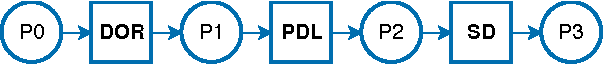
\includegraphics[width=0.37\linewidth]{content/figures/pharmaDep1.pdf}\label{fig:wfnet:a}}
%	\hfill
%	\subfloat[][Specialized clinic's log.]{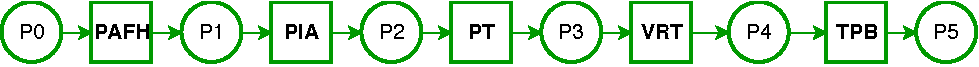
\includegraphics[width=0.57\linewidth]{content/figures/specialisedDep1.pdf}\label{fig:wfnet:b}}
%	\hfill
%	\vspace{1em}
%	\subfloat[][Hospital's log.]{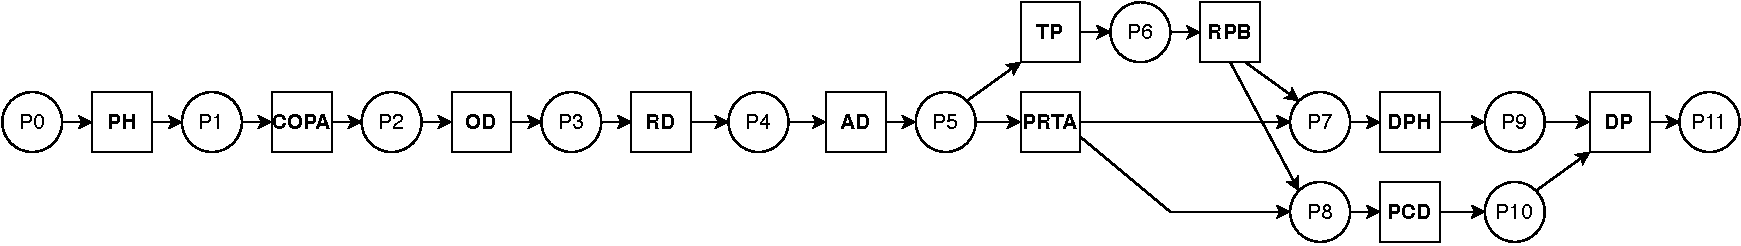
\includegraphics[width=1\linewidth]{content/figures/hospitalDep1.pdf}\label{fig:wfnet:c}}
%	\hfill
%	\vspace{1em}
%	\subfloat[][Full log, merged via the CONFINE protocol.]
	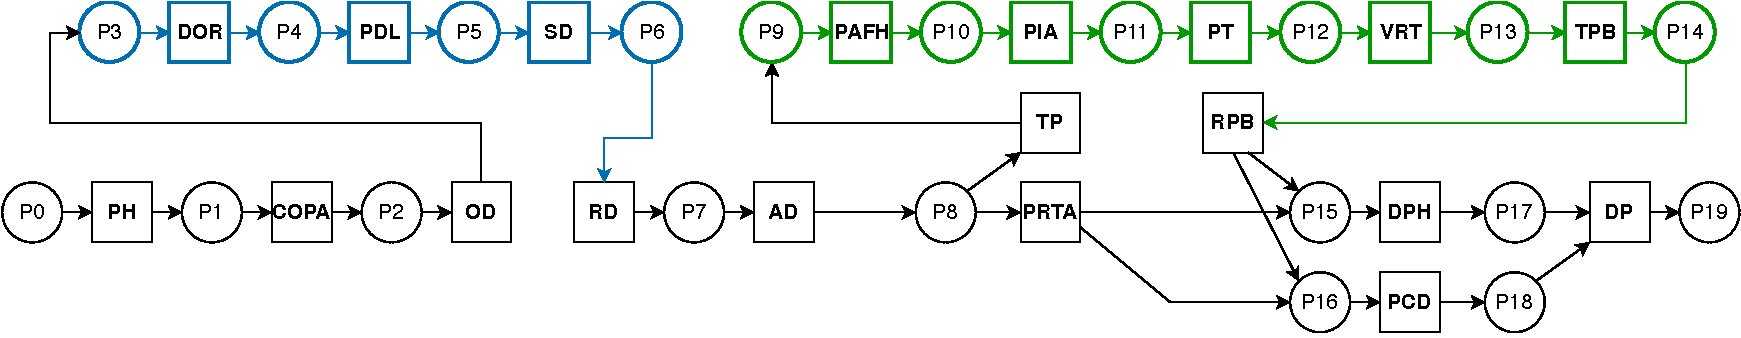
\includegraphics[width=1\linewidth]{content/figures/mergedDep1.pdf}\label{fig:wfnet:d}
	\caption[HeuristicsMiner output]{\emph{HeuristicsMiner} output in CONFINE}
	\label{fig:wfnet}
\end{figure}    


\noindent\textbf{Output convergence.}
\label{sec:evaluation:subsec:convergence}
%We assess the convergence of the \textit{HeuristicsMiner} outcomes as a means of validating the correct functioning of the event log transmission mechanism. 
To experimentally validate the correctness of our approach in the transmission and computation phases (see \cref{sec:realization}), we run a \emph{convergence} test. %Specifically, we generated workflow net outputs by applying intra-organizational mining procedures, wherein each organization independently mined its event log. Subsequently, we employed our approach with a miner actor conducting the \textit{HeuristicsMiner} algorithm using an inter-organizational event log obtained as a result of the log exchange and merging mechanisms. Finally, we compared the results obtained through our approach with the single outputs mined using the partial event log in intra-organizational setting.  
To this end, we created a synthetic event log consisting of \num{1000} cases of \num{14} events on average (see \cref{tab:testedlogs}) by simulating the inter-organizational process of our motivating scenario 
(see \cref{fig:BPMN_Healthcare})%
%
\footnote{We generated the event log through BIMP (\url{https://bimp.cs.ut.ee/}). We filtered the generated log by keeping the sole events that report on the completion of activities, and removing the start and end events of the \Actor{Pharmaceutical company} and \Actor{Specialized clinic}'s sub-processes.}
%
and we partitioned it in three sub-logs (one per involved organization), an excerpt of which is listed in~\cref{tab:trace}.
We run the stand-alone \textit{HeuristicsMiner} on the former, and processed the latter through our CONFINE toolchain.
As expected, the results converge and are depicted in \cref{fig:wfnet} in the form of a workflow net~\citep{Aalst/ICATPN97:VerificationofWfNs}. For clarity, we have colored activities recorded by the organizations following the scheme of~\cref{tab:testedlogs} (black for the \Actor{Hospital}, blue for the \Actor{Pharmaceutical company}, and green for the \Actor{Specialized clinic}).
%Upon careful examination of \cref{fig:wfnet}, we show that the workflow net generated by the \textit{HeuristicsMiner} in our approach, as displayed in \cref{fig:wfnet:d}, encapsulates the structure and behavior observed in the workflow nets produced by the intra-organizational \textit{HeuristicsMiner} execution. In specific terms, the blue-colored part in \cref{fig:wfnet:d} reflects the behavior of the \Actor{Pharmaceutical company}, depicted in \cref{fig:wfnet:a}, commencing from the moment the drug order is received to its fulfillment. Furthermore, the green-colored part delineates the process of the \Actor{Specialized clinic}, starting from the patient's arrival from the \texttt{Hospital} to their transfer described in \cref{fig:wfnet:b}. Finally, the black-colored portion of the workflow net is consistent with the output resulting from the partial log of the \Actor{Hospital} showed in \cref{fig:wfnet:c}.
%Event logs and formula tables
%

\begin{figure}[t]
\centering
\begin{subfigure}{0.49\textwidth}
  \centering
  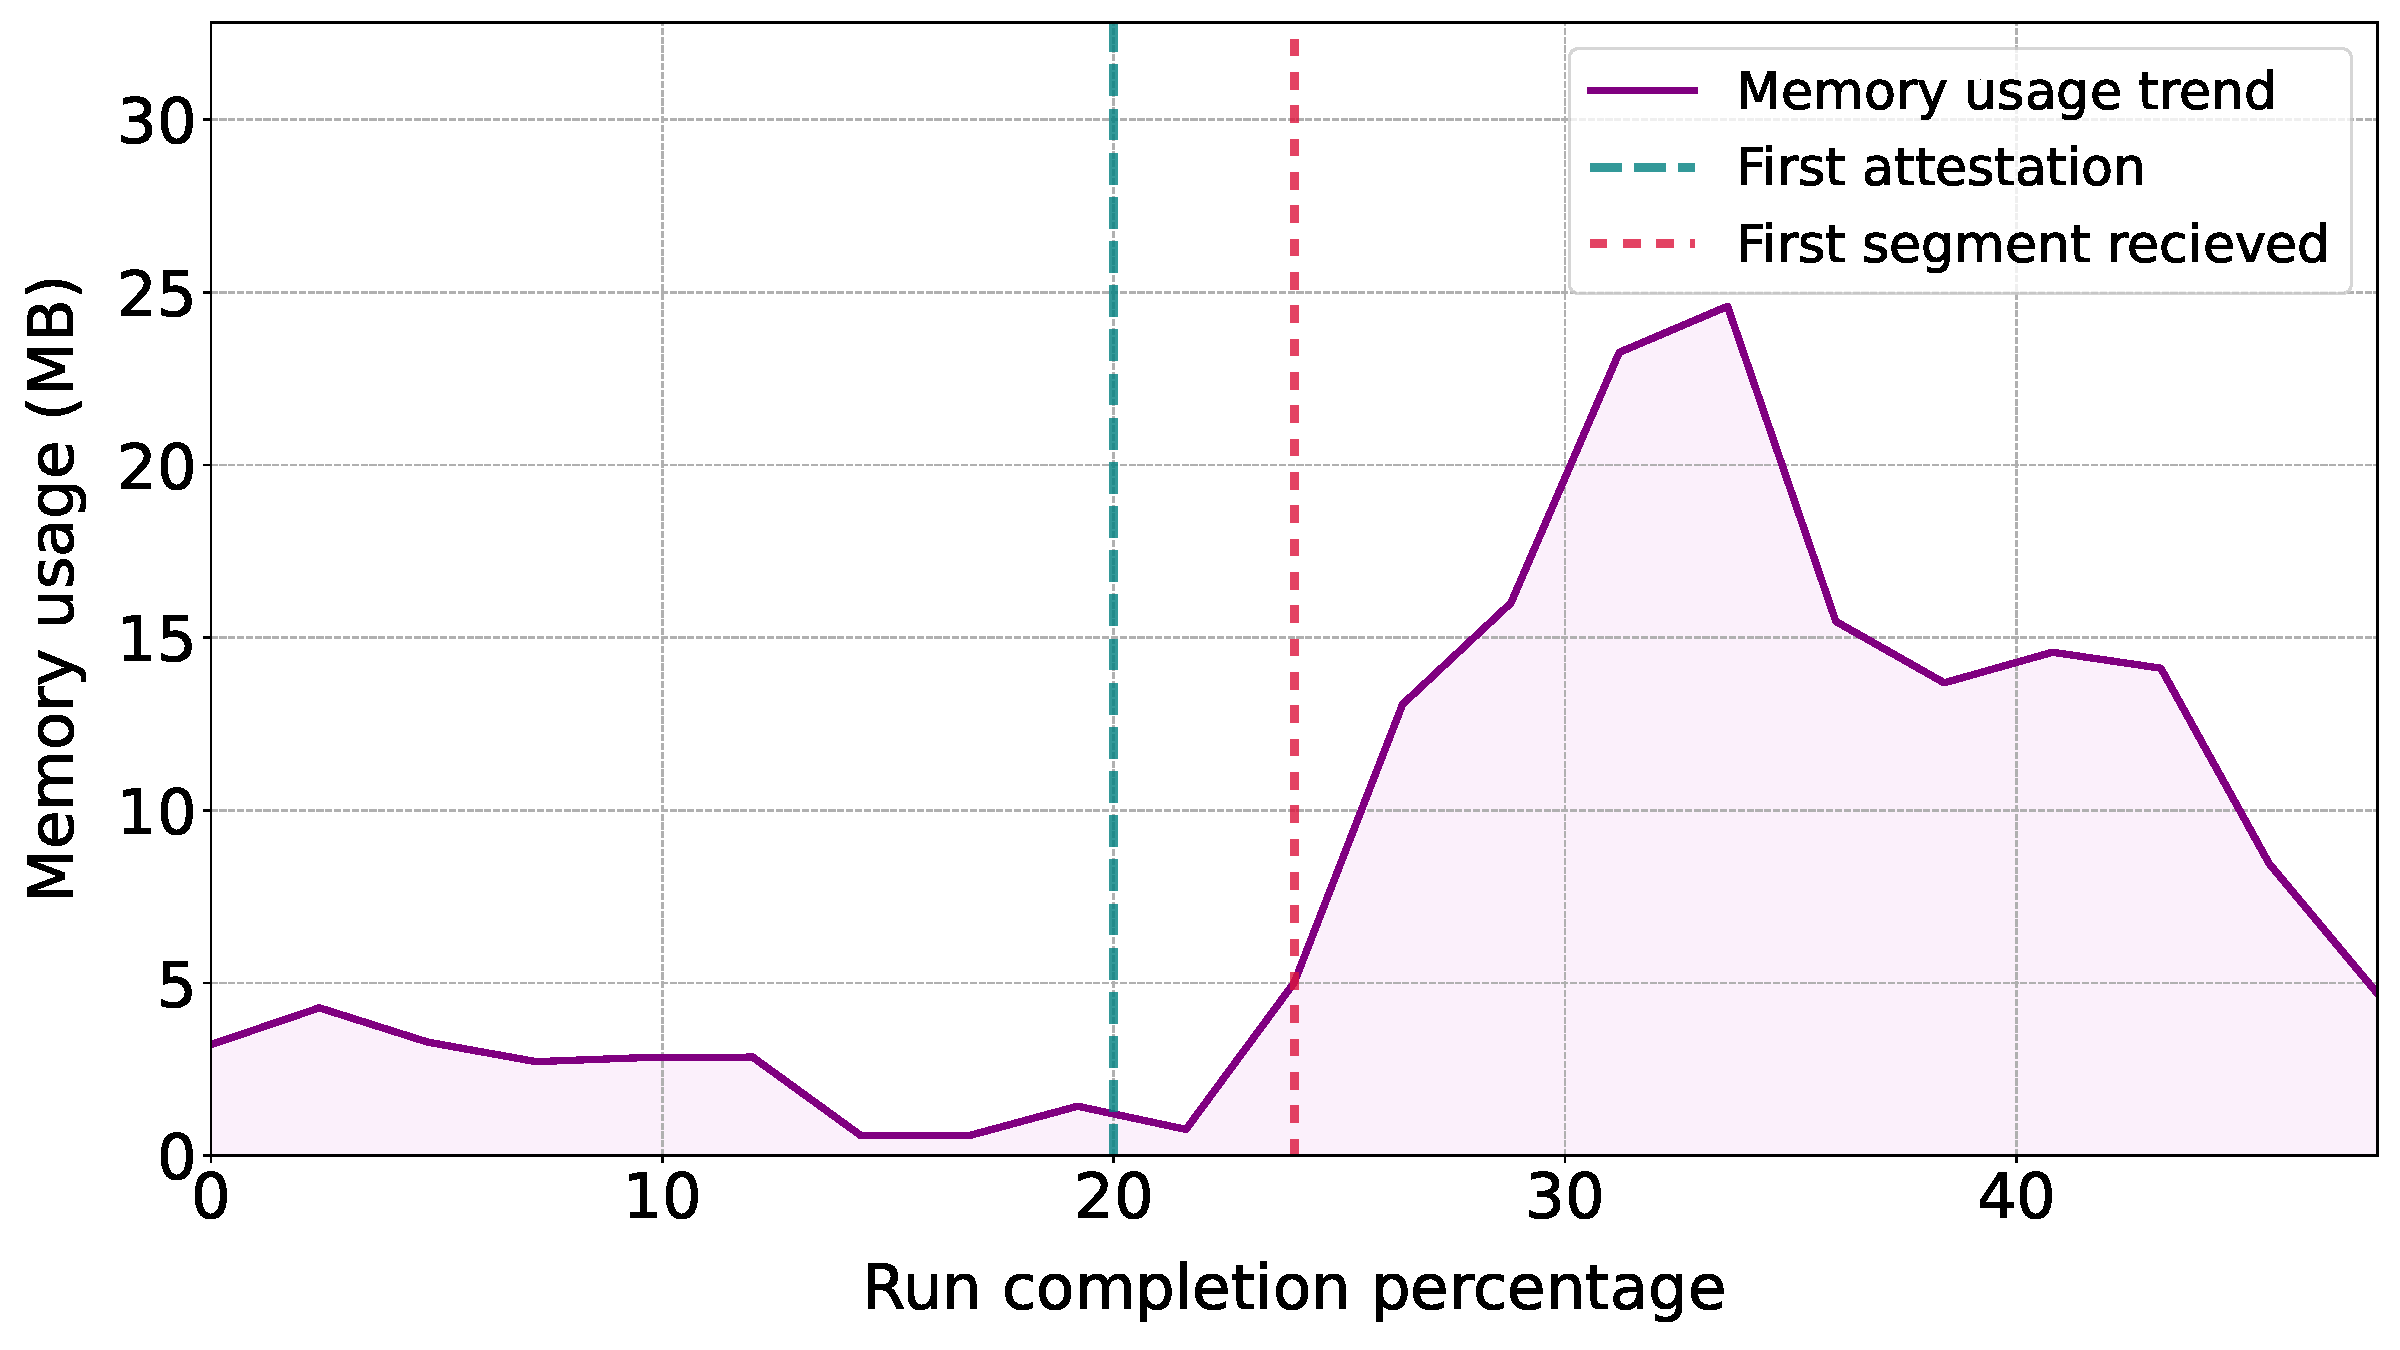
\includegraphics[width=\textwidth]{content/figures/memoryusage1-2.pdf}
  \caption{Memory usage without the computation phase}
  \label{snr_a}
\end{subfigure}\hfill
\begin{subfigure}{0.49\textwidth}
  \centering
  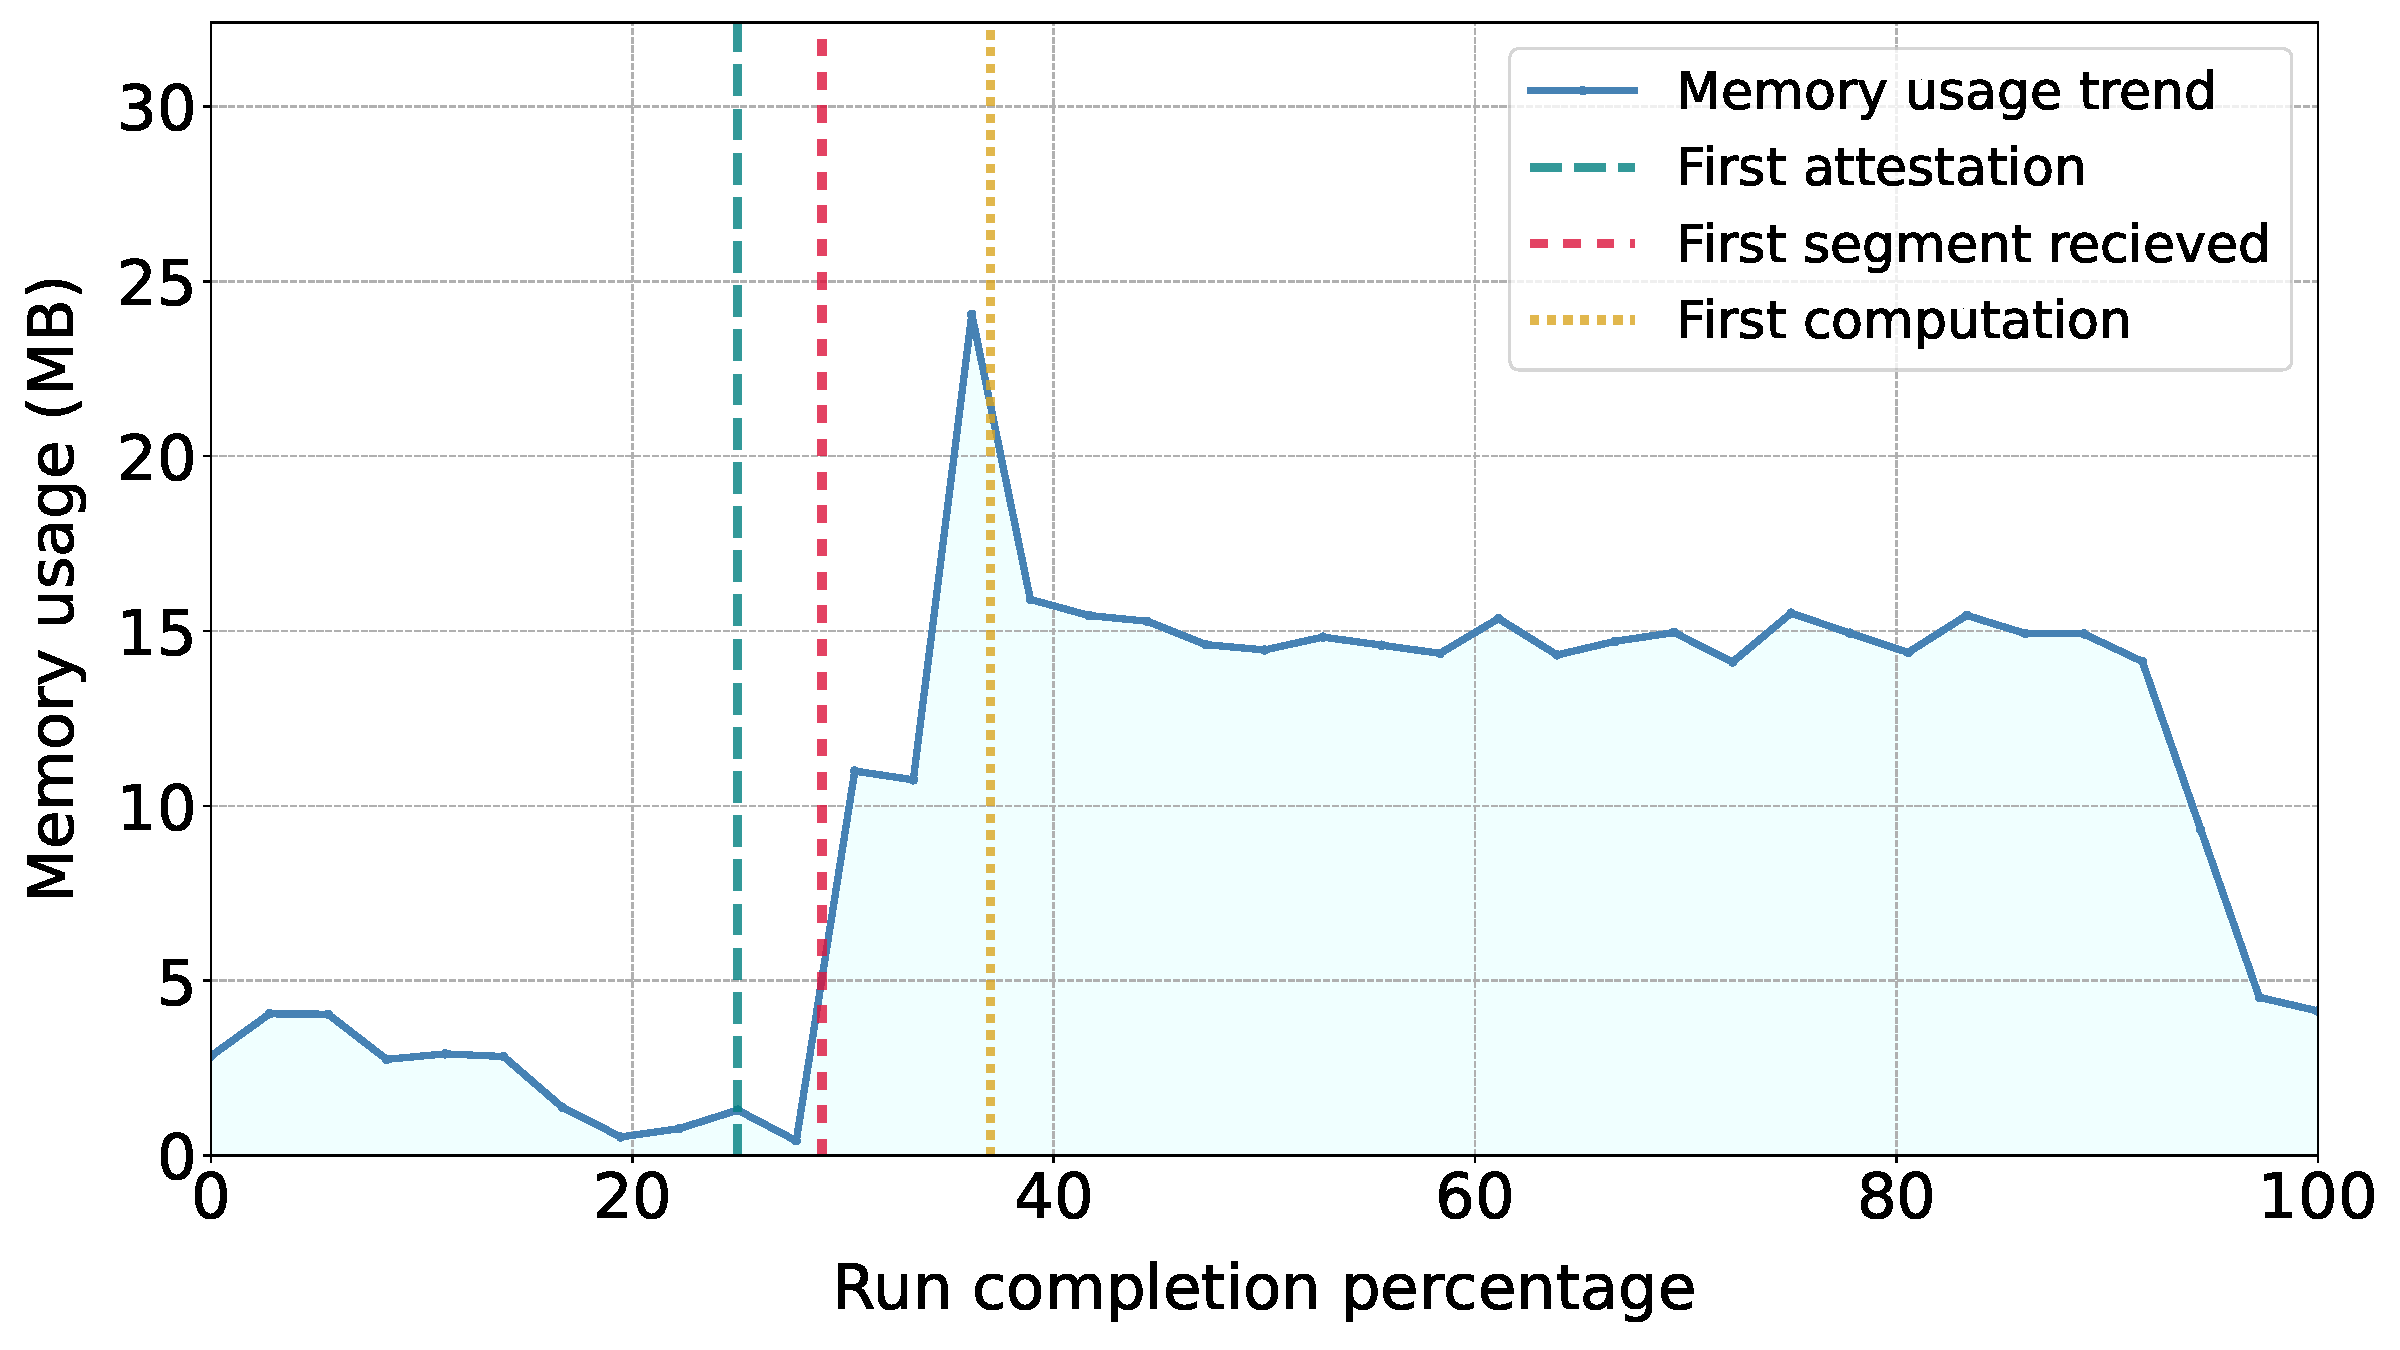
\includegraphics[width=\textwidth]{content/figures/memoryusage2-2.pdf}
  \caption{Memory usage with the computation phase}
  \label{snr_b}   
\end{subfigure}

\begin{subfigure}{0.49\textwidth}   
  \centering      
  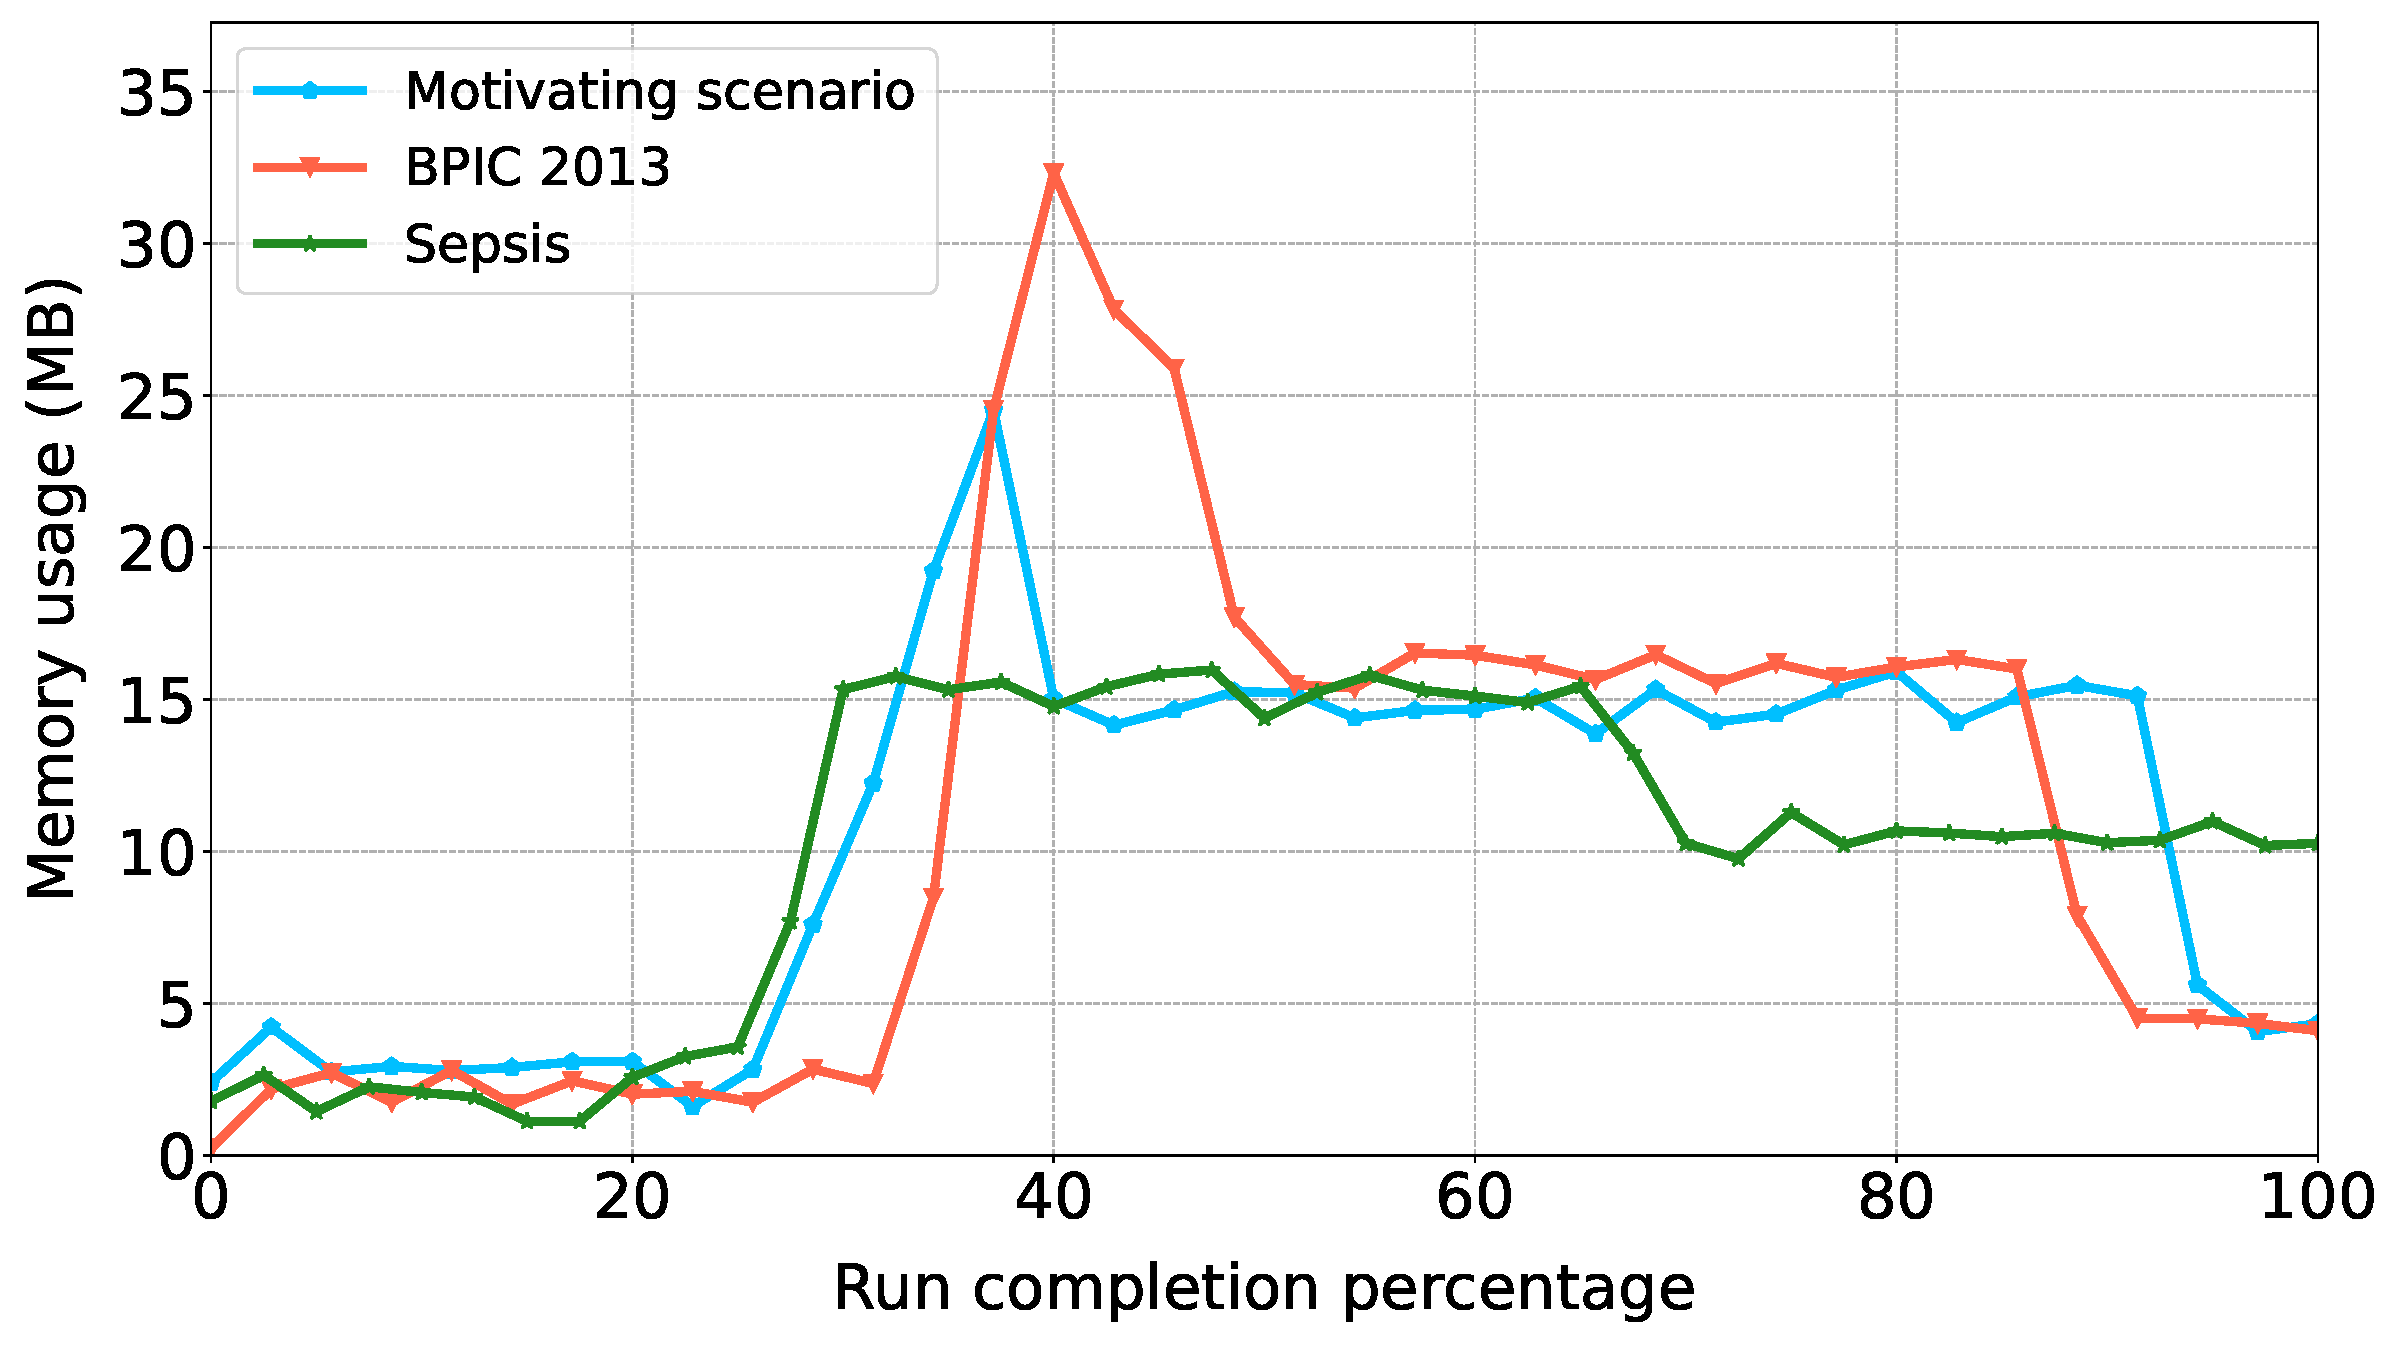
\includegraphics[width=\textwidth]{content/figures/memoryusage3-2.pdf}
  \caption{Memory usage comparison with three event logs}
  \label{snr_c}
\end{subfigure}
\begin{subfigure}{0.49\textwidth}   
  \centering
  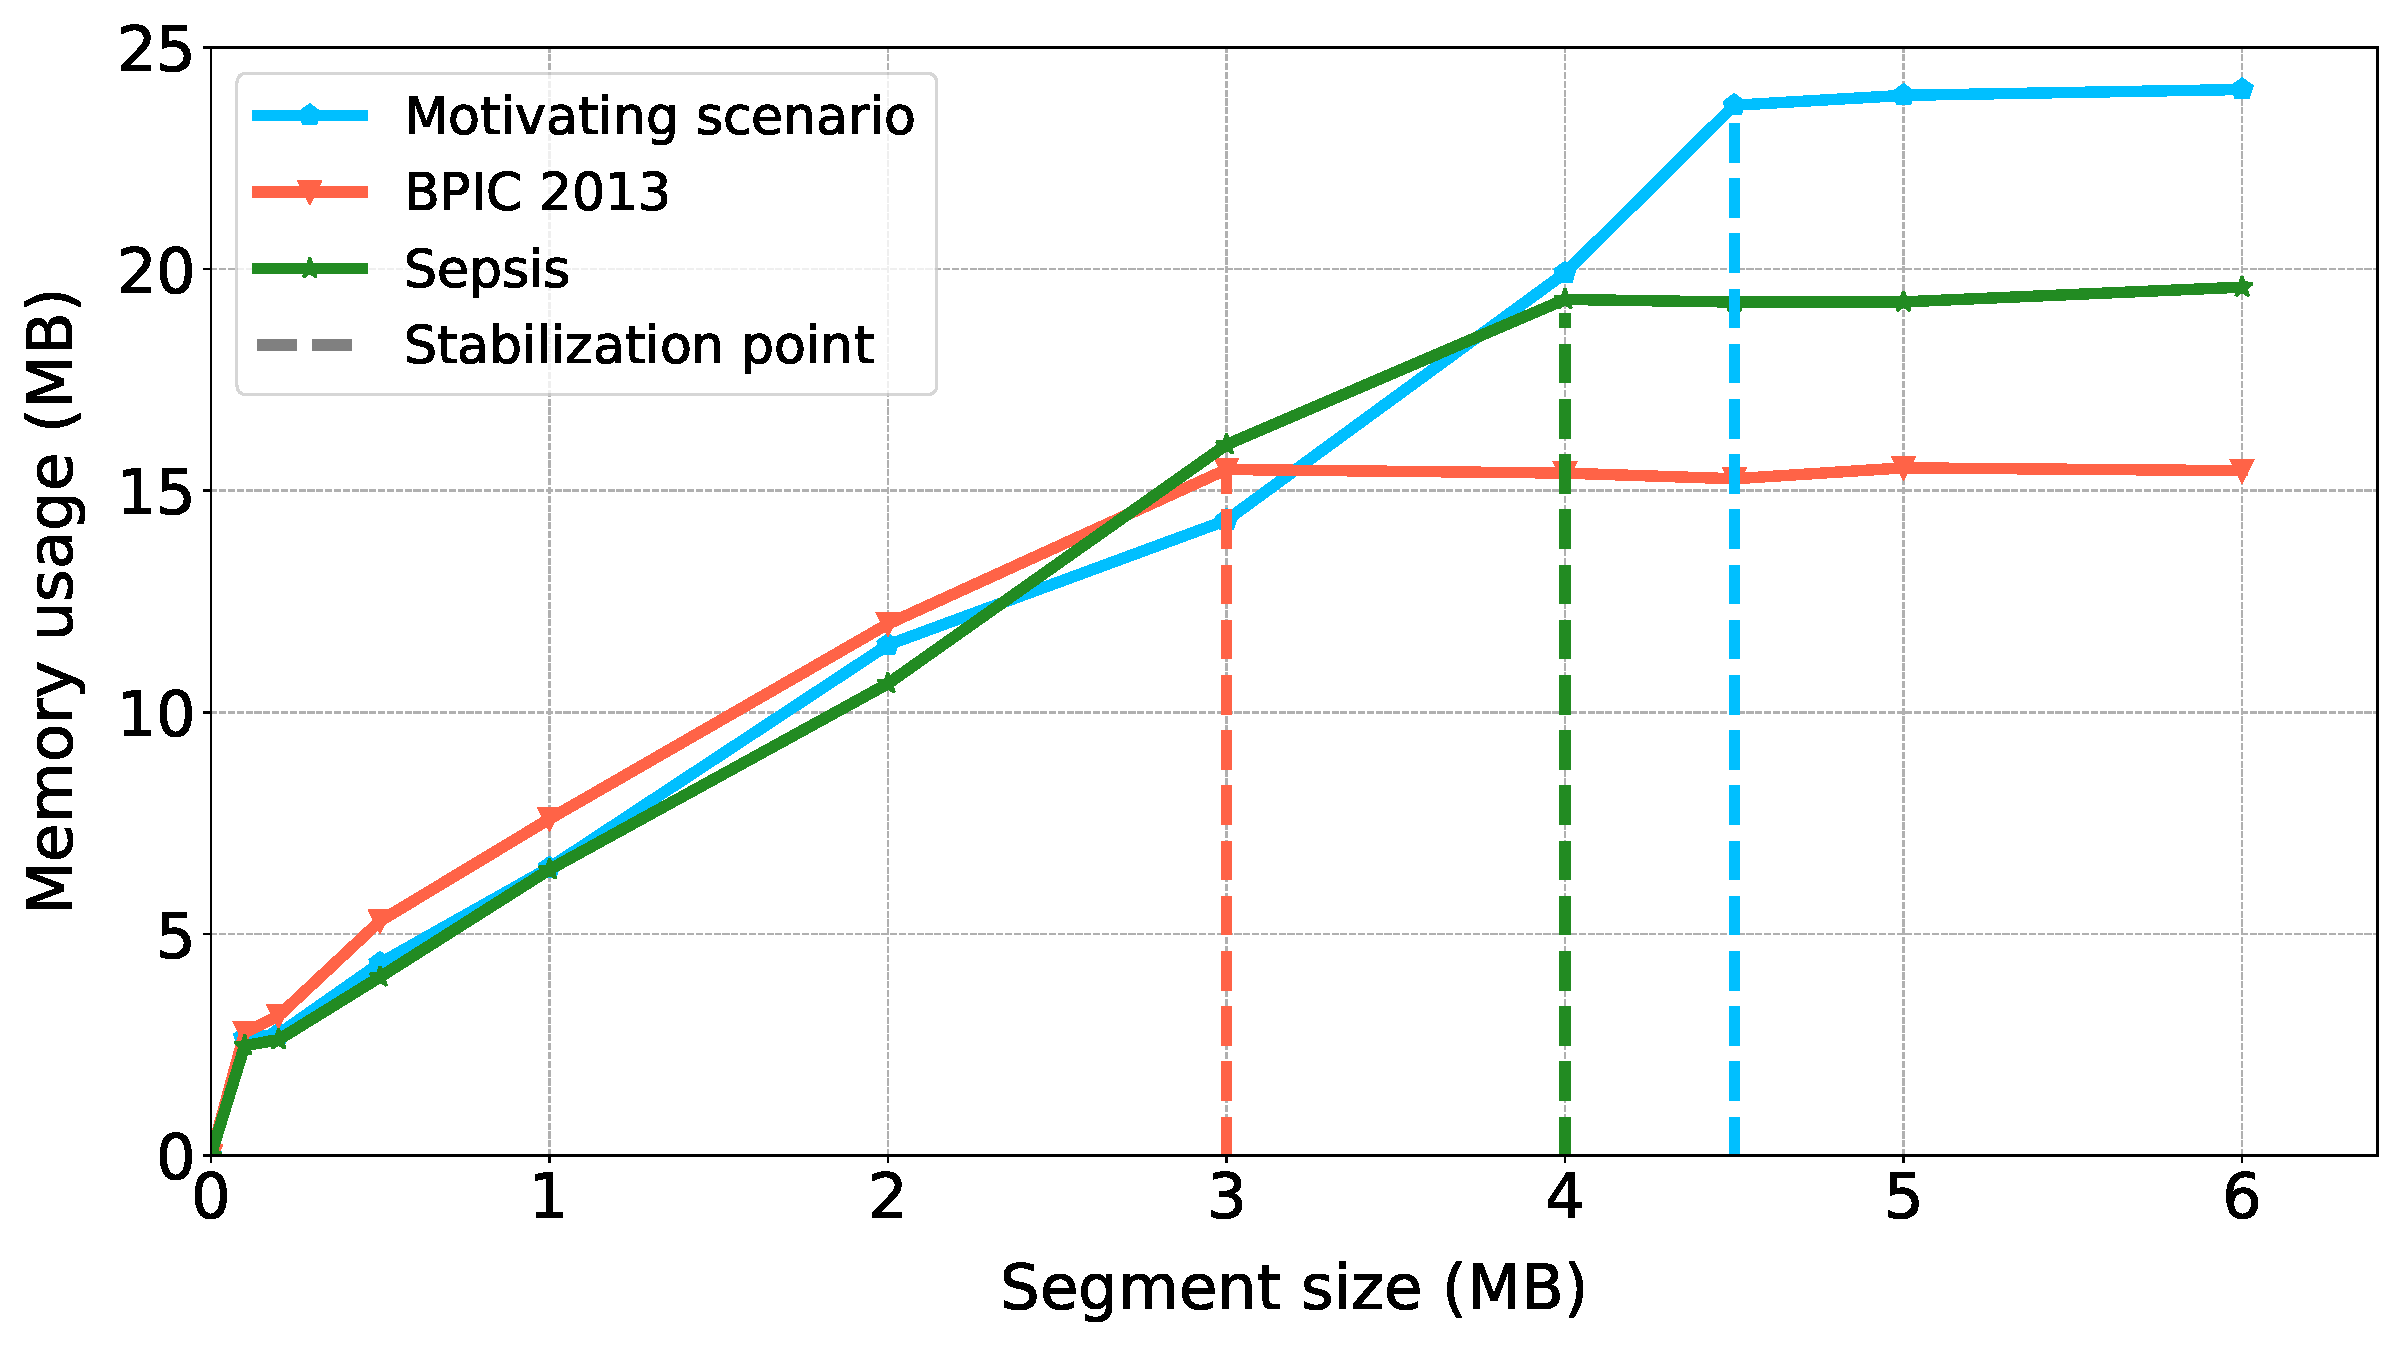
\includegraphics[width=\textwidth]{content/figures/memoryusage4-2.pdf}
  \caption{Segment size impact on memory usage}
  \label{snr_d}
\end{subfigure}
\caption{Memory usage test results}
\label{fig:memtest}
\end{figure}

\noindent\textbf{Memory usage.} \label{sec:evaluation:subsec:MemoryUsage} \Cref{snr_a,snr_b} display plots corresponding to the runtime memory utilization of our CONFINE implementation (in MegaBytes). Differently from \cref{snr_b}, \cref{snr_a} excludes the computation stage by leaving the \emph{HeuristicsMiner} inactive so as to isolate the execution from the mining-specific operations. %phases an execution where the Heuristics Miner algorithm remained inactive. The 
The dashed lines mark %purple line illustrates the trend of memory usage (in MegaBytes), during the execution, while the two lines mark 
the starting points for the remote attestation, the data transmission and the computation stages. %receiving of event log segments sent by the providers, indicated by the green and the red dotted line, respectively. In this examination, 
We held the {\SegSize} constant at \num{2000} KiloBytes. % and utilized the Motivating Scenario event log. To emphasize the transmission and reception of event logs with the greatest data volume, we designated the \Actor{Specialized clinic} as the miner due to the lower weight of its corresponding event log. \Actor{Hospital} and \Actor{Pharmaceutical company} served as the two providers.\cref{snr_b} reveals that the initial computation by the \textit{HeuristicsMiner} algorithm, depicted by the orange dashed line, commences immediately after the conclusion of the segment reception phase. 
We observe that the data transmission stage reaches the highest peak of memory utilization, % concludes approximately at the initiation of the first computation, 
which is then partially freed by the subsequent computation stage, steadily occupying memory space at a lower level. %which absorbs a substantial portion of the resources utilized 
%throughout .
To verify whether this phenomenon is due to the synthetic nature of our simulation-based event log, we also gauge the runtime memory usage of two public real-world event logs too (Sepsis~\citep{seps} and BPIC 2013~\citep{bpic2013}). %from existing literature. As shown in \cref{tab:testedlogs}, we selected similar event logs based on the number of cases and overall weight to facilitate a meaningful comparison.
The characteristics of the event logs are summarized in \cref{tab:testedlogs}.
Since those are \textit{intra-organizational} event logs, we %have resorted to modifications to make the log matching to an \textit{inter-organizational} context. 
split the contents to mimic an \textit{inter-organizational} context.
In particular, we separated the Sepsis event log based on the distinction between normal-care and intensive-care paths, as if they were conducted by two distinct organizations. Similarly, we processed the BPIC~2013 event log to sort it out into the three departments of the Volvo IT incident management system. % For each scenario, we designated the actor with the smallest log size as the miner to maximize the exchanged data volume. %Clearly, the 
\Cref{snr_c} depicts the results. We observe that the processing of the BPIC 2013 event log demands more memory, particularly during the initial stages, probably owing to its larger size. Conversely, the Sepsis event log turns out to entail the least expensive run. %, with the least memory consumption and a well-balanced profile. 
To verify whether these trends are affected by the dimension of the exchanged data segments, we conducted an additional test to examine the trend of memory usage as the {\SegSize} varies with all the aforementioned event logs. %In this configuration, we used the same three event logs mentioned above with identical settings. 
Notably, the polylines displayed in \cref{snr_d} indicate a linear increment of memory occupation until a breakpoint is reached. After that, the memory in use is steady. These points, marked by vertical dashed lines, correspond %where the execution reaches a maximum memory usage value, corresponding 
to the {\SegSize} value that allows the provider's segments to be contained in a single data segment.

\begin{comment}
\begin{wrapfigure}[8]{r}{0.40\textwidth}
        \vspace{-2.9em}
            \renewcommand{\arraystretch}{2.5}
            \begin{tabular}{l}
            %(a) \resizebox{0.9\textwidth}{!}{$\LinearCorrelationCoefficent = \LinearCorrelationCoefficentF$}\phantomsubcaption\label{formula:pearson}\\ 
            (a) %\resizebox{0.9\textwidth}{!}
            {$\RCoefficent = \RCoefficentF$}\phantomsubcaption\label{formula:r2}\\
            (b) %\resizebox{0.9\textwidth}{!}
            {$\Slope = \SlopeF$}\phantomsubcaption\label{formula:angCoefficent}\\
            %(c) \resizebox{0.75\textwidth}{!}{$\RCoefficent = \RCoefficentF$}\phantomsubcaption\label{formula:r2}\\
            \end{tabular}
        \vspace{-0.2em}
        \caption{Formulas used in the scalability test analysis}
        \label{formula}
\end{wrapfigure}
\end{comment}

\begin{comment}

\begin{figure}[ht!]
\centering
\begin{subfigure}{0.49\textwidth}
  \centering
  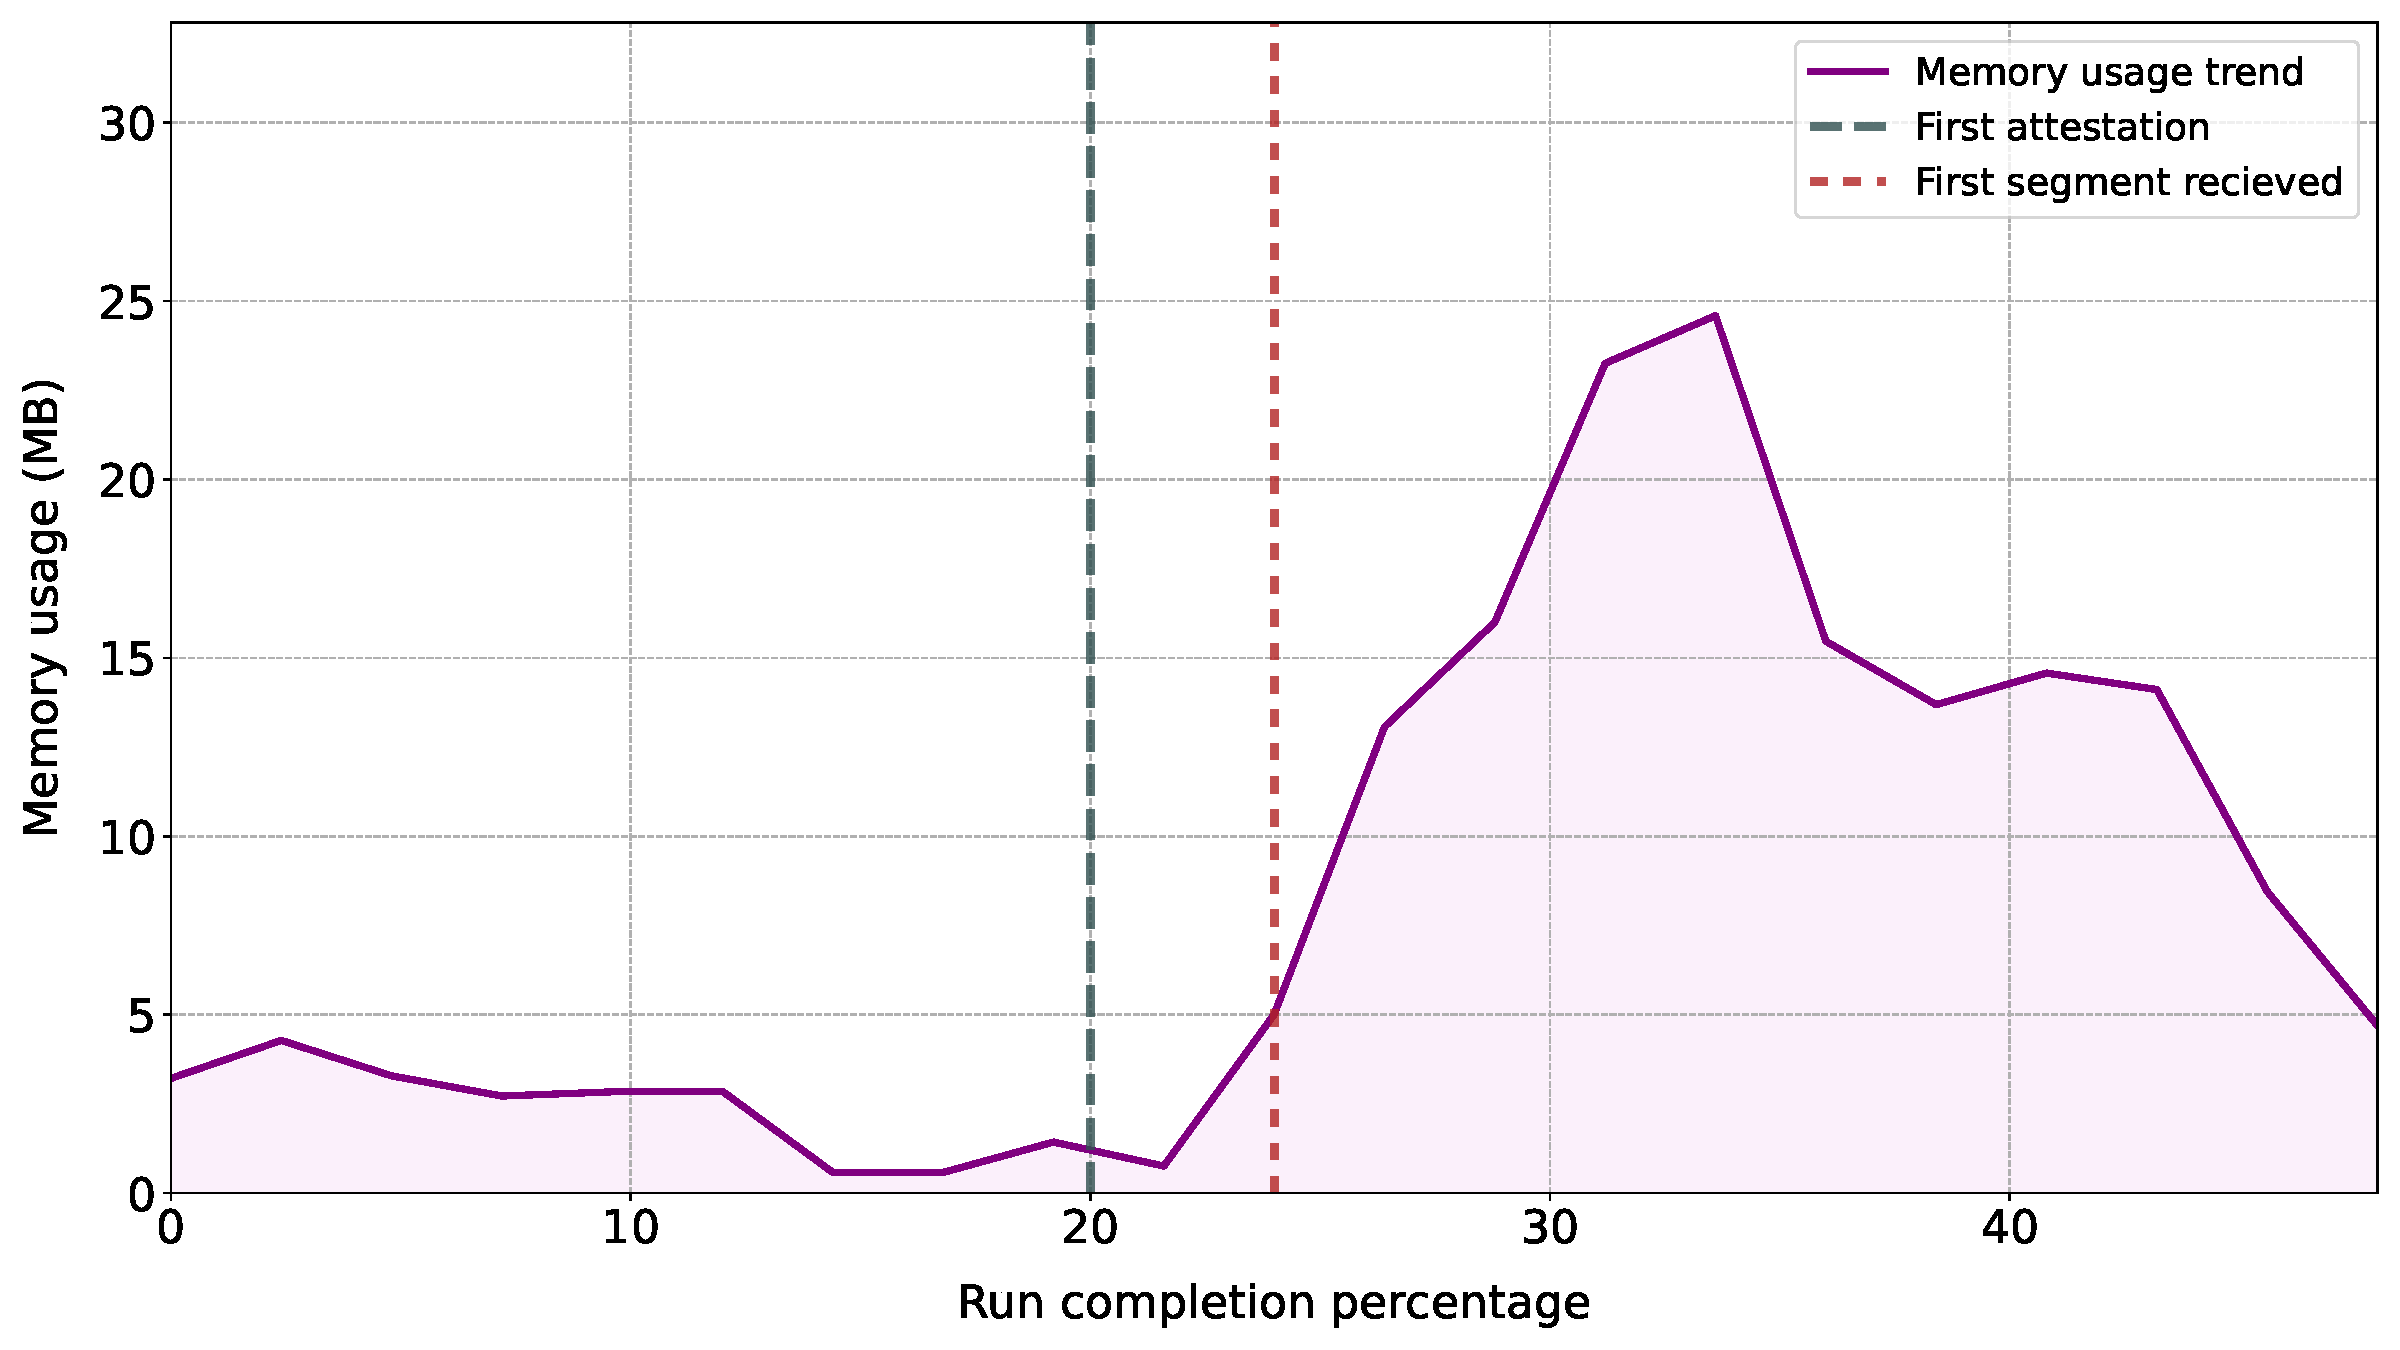
\includegraphics[width=\textwidth]{content/figures/memoryusage1.pdf}
  \caption{to be replaced with the single event log version with mark lines.}
  \label{snr_a}
\end{subfigure}\hfill
\begin{subfigure}{0.49\textwidth}
  \centering
  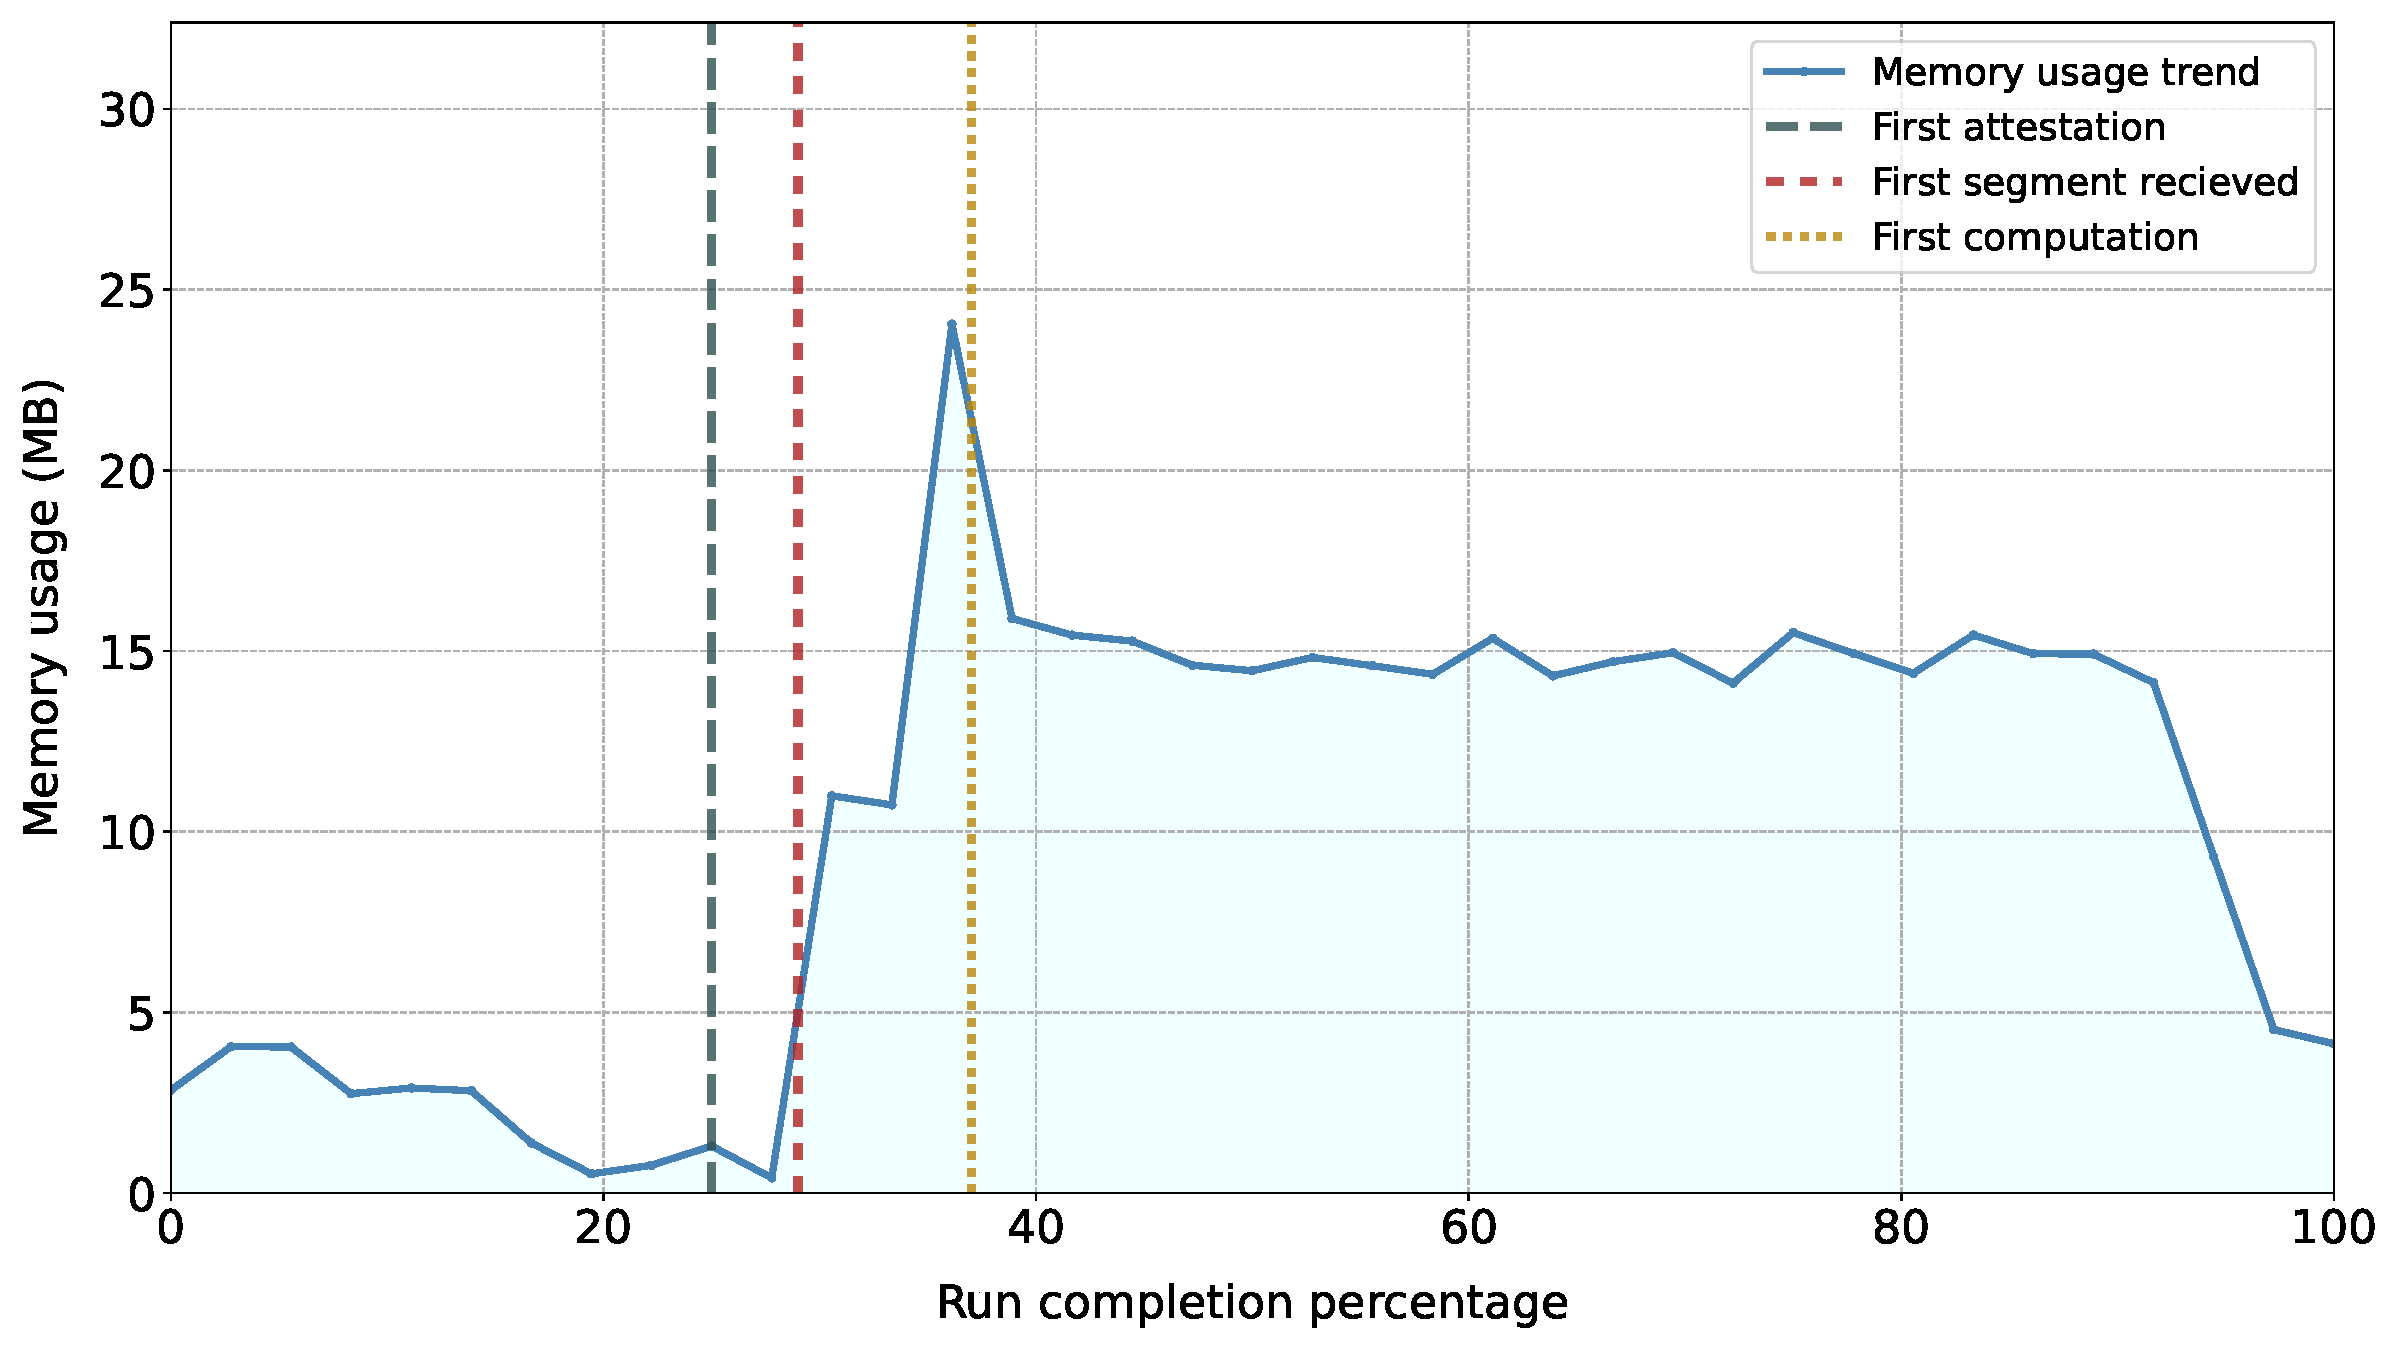
\includegraphics[width=\textwidth]{content/figures/memoryusage2.pdf}
  \caption{Ram usage at run time for three event logs.}
  \label{snr_b}   
\end{subfigure}

\begin{subfigure}{0.49\textwidth}   
  \centering      
  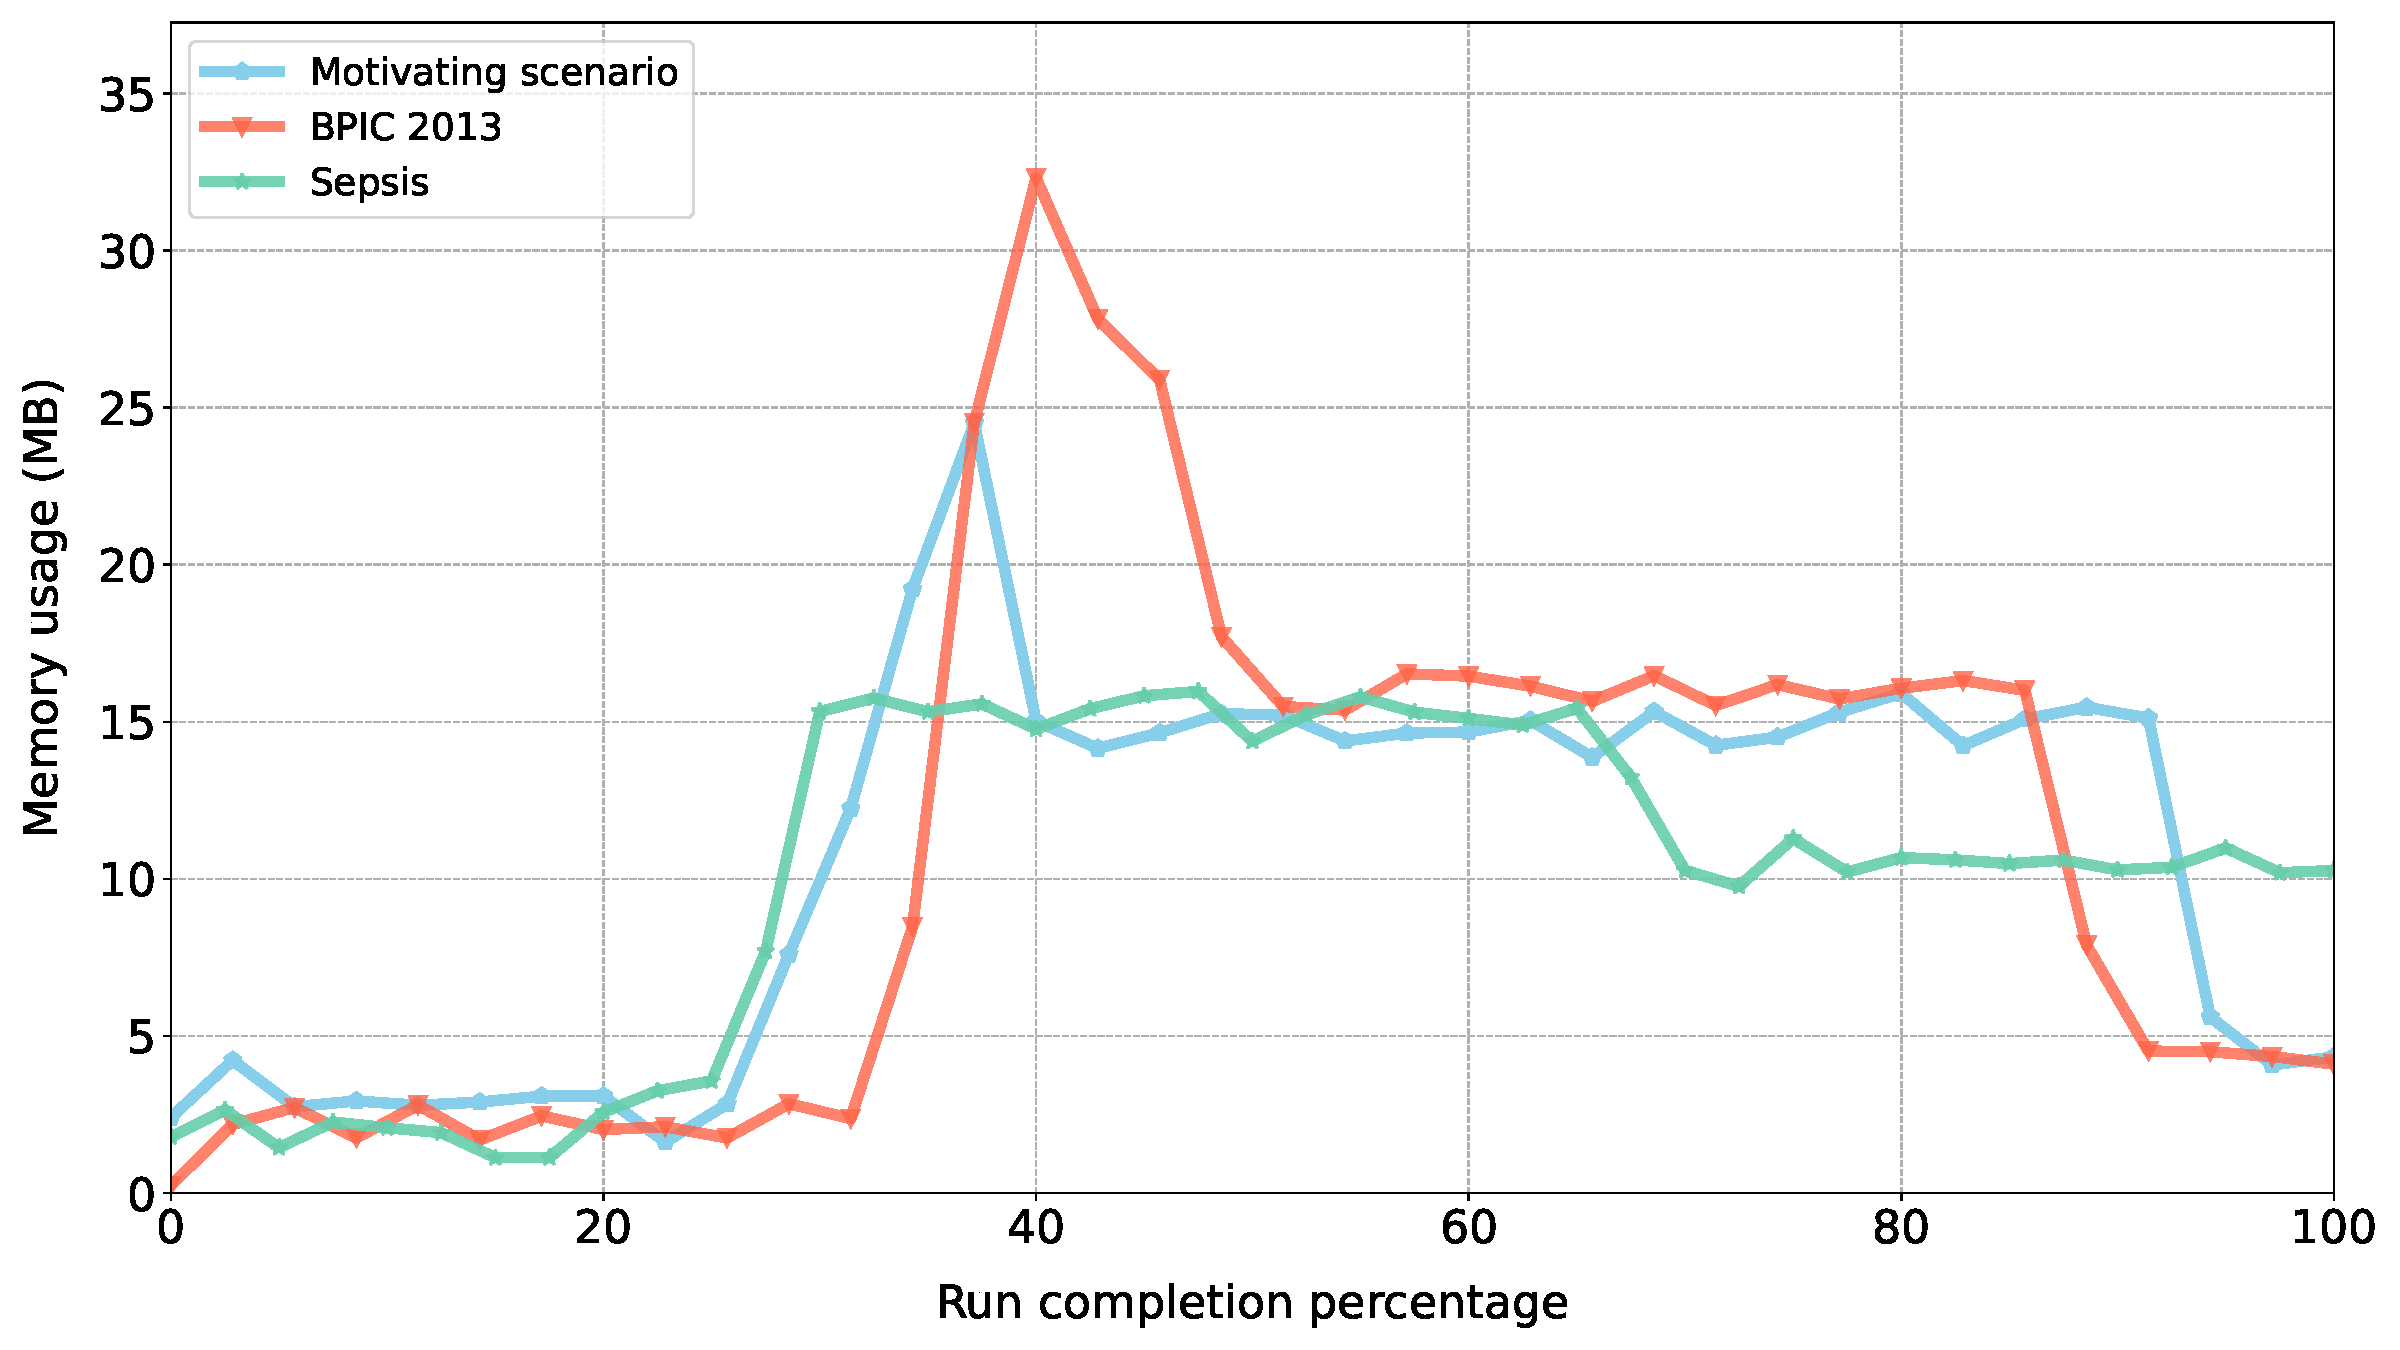
\includegraphics[width=\textwidth]{content/figures/memoryusage3.pdf}
  \caption{Memory usage as segment size increases}
  \label{snr_c}
\end{subfigure}
\begin{subfigure}{0.49\textwidth}   
  \centering
  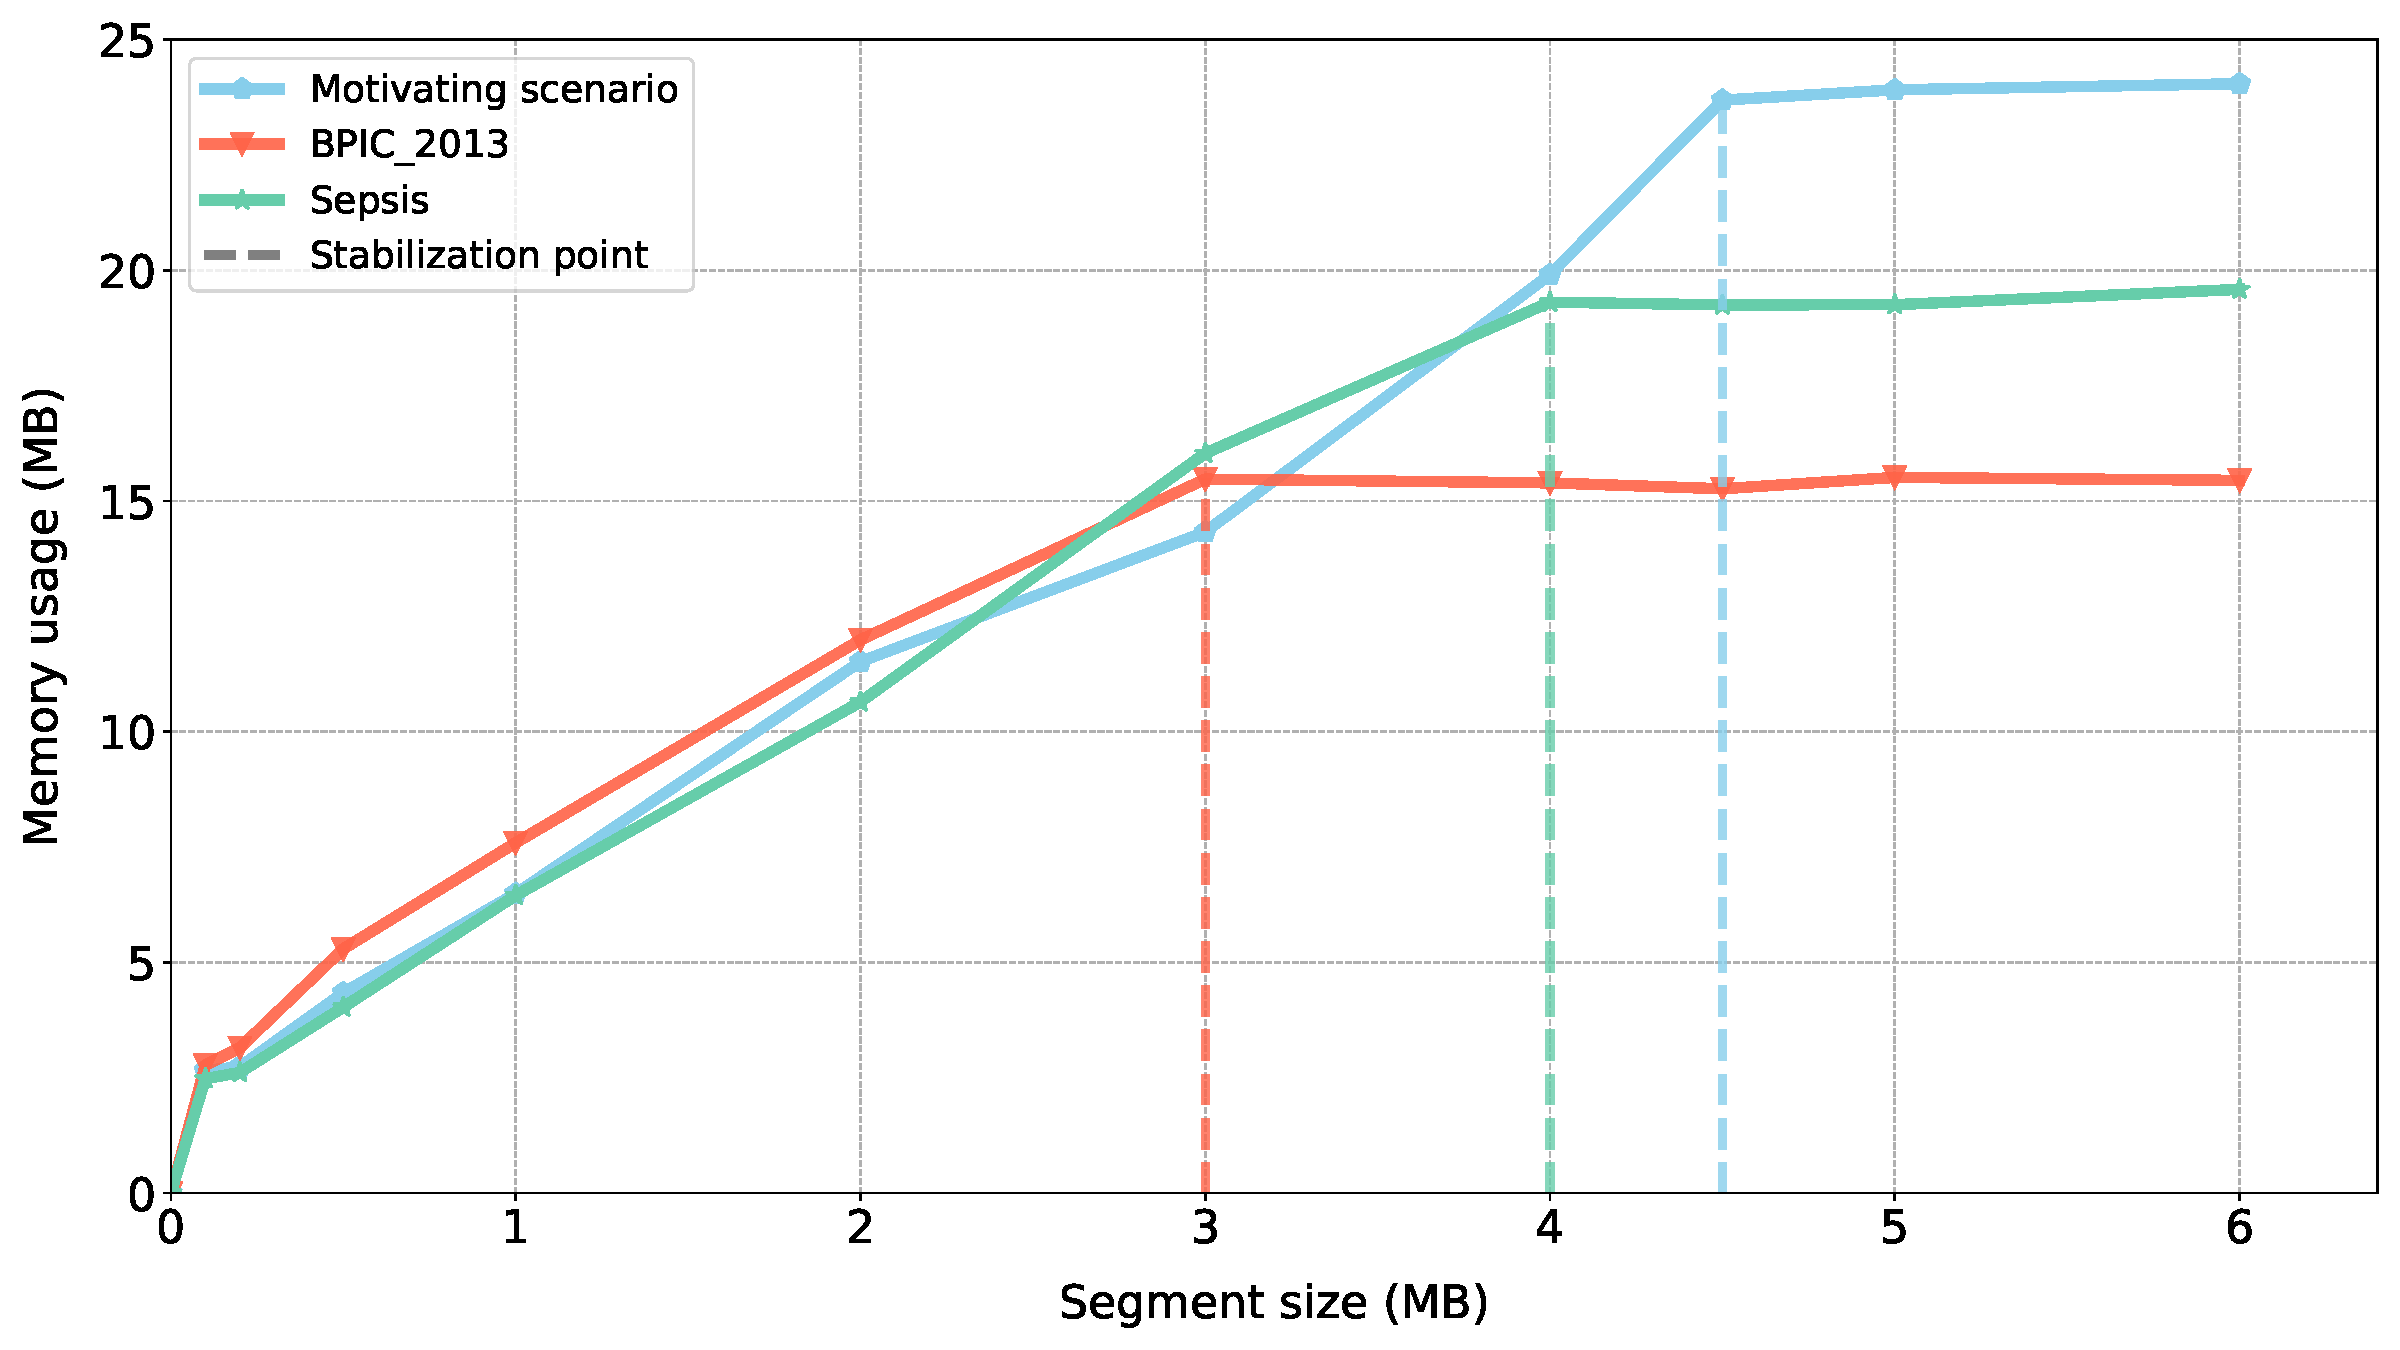
\includegraphics[width=\textwidth]{content/figures/memoryusage4.pdf}
  \caption{to be replaced with scalability test}
  \label{snr_d}
\end{subfigure}

\begin{subfigure}{0.49\textwidth}   
  \centering
  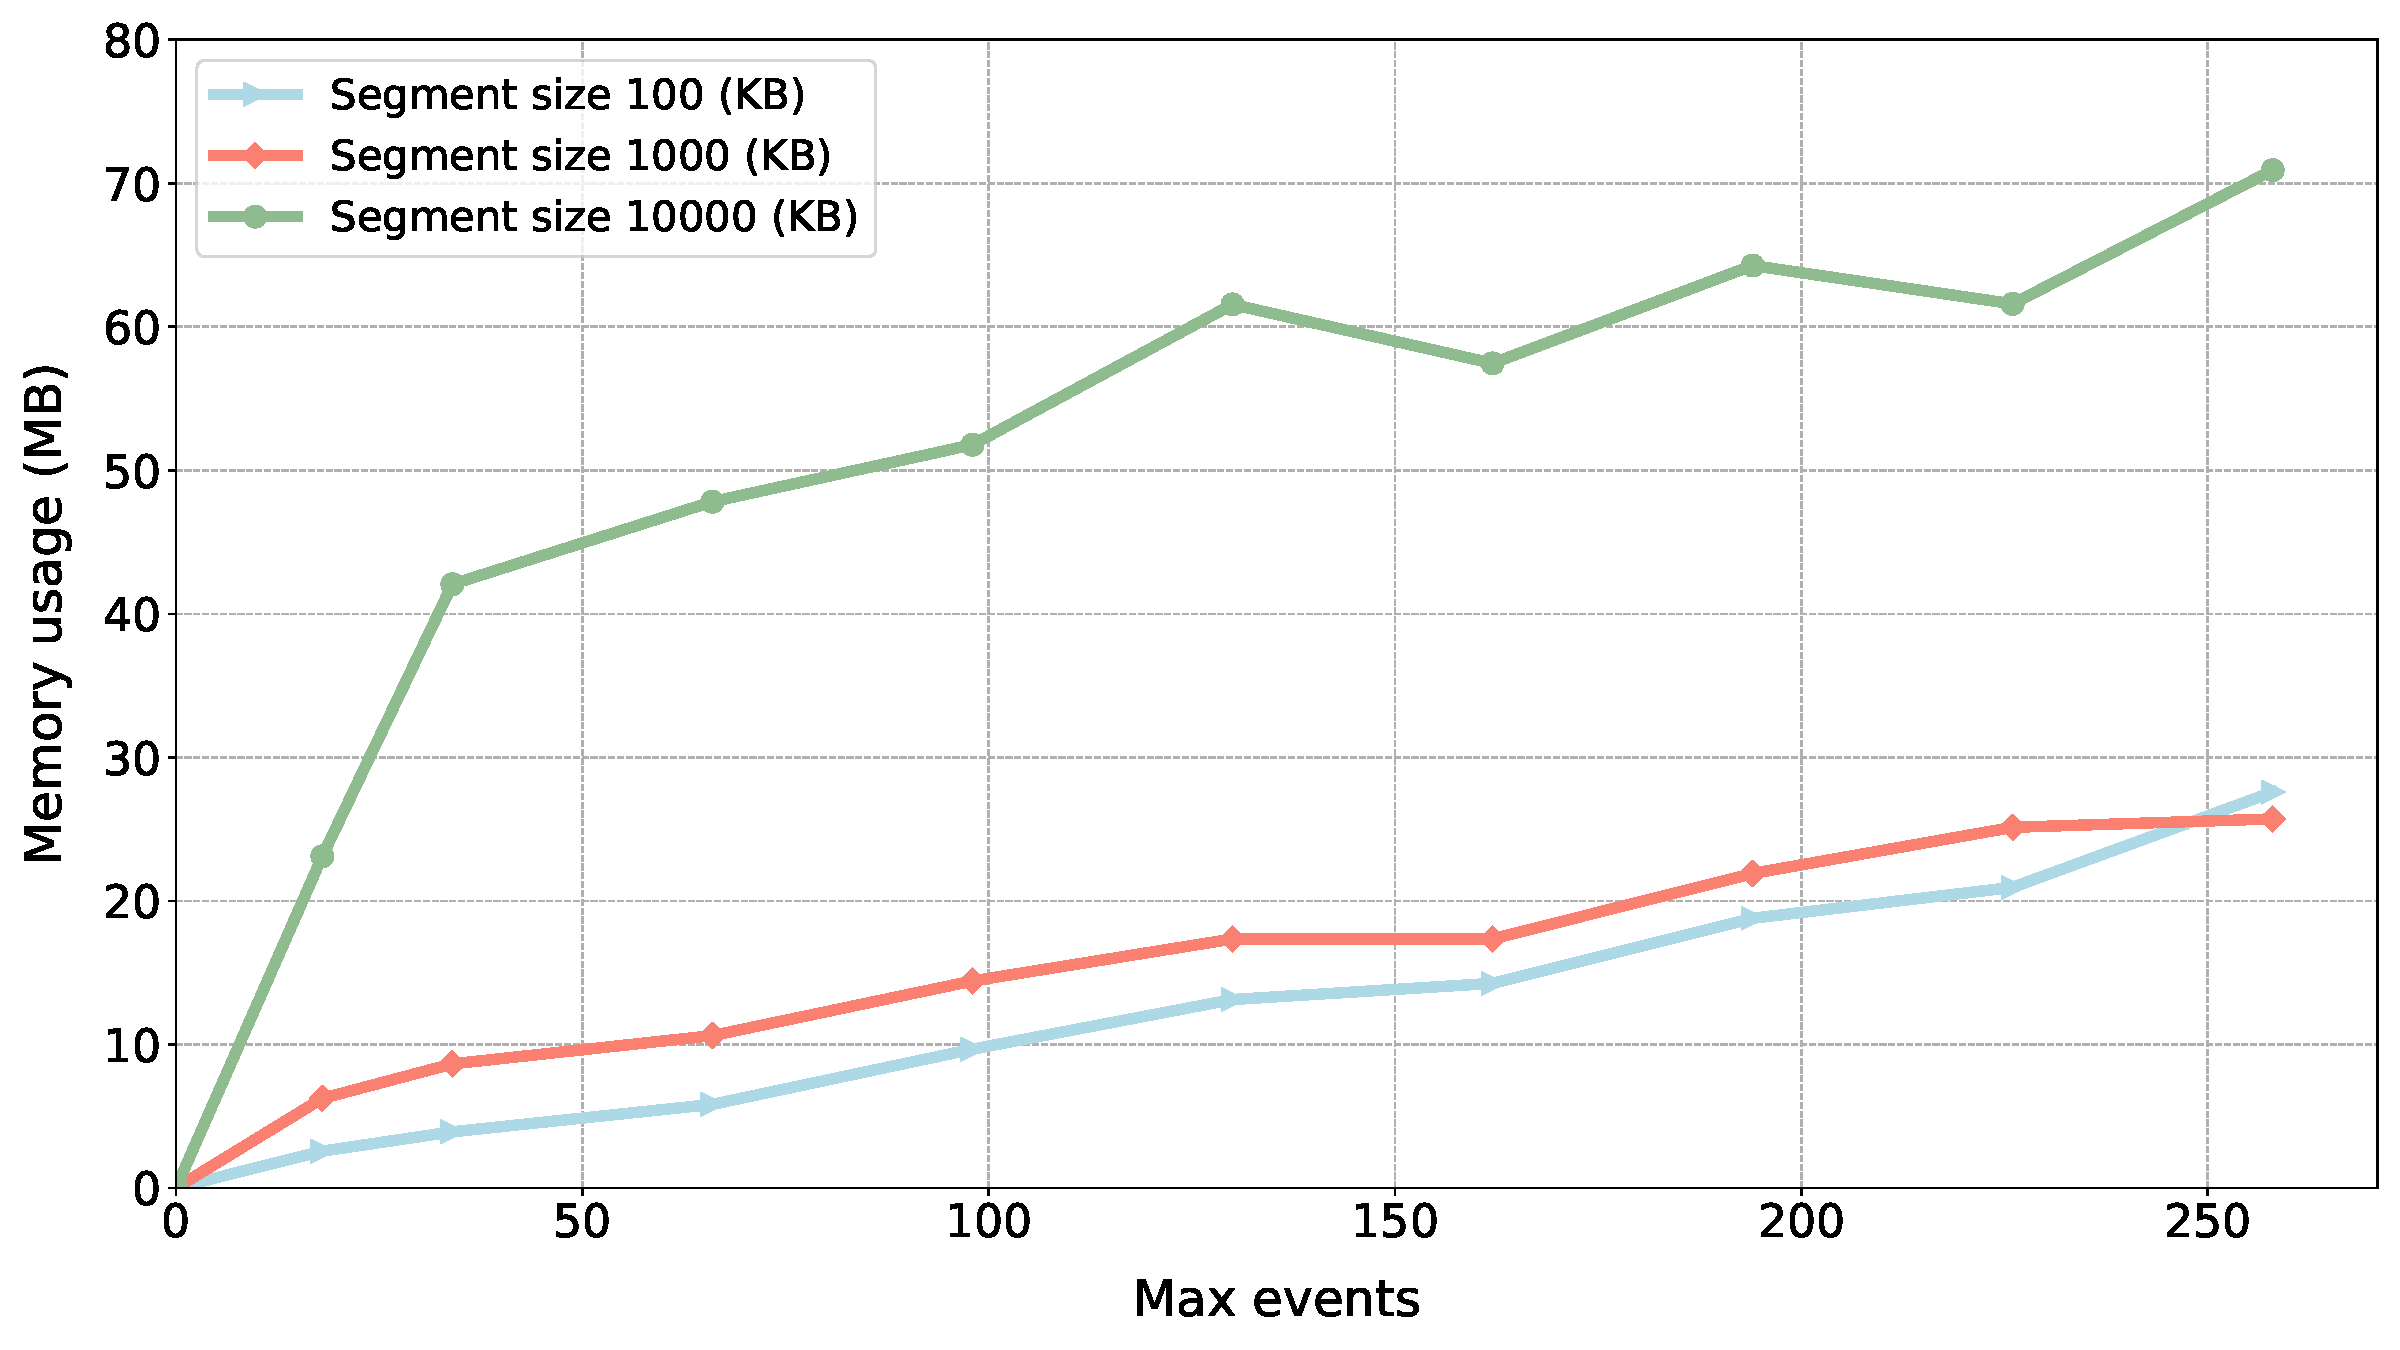
\includegraphics[width=\textwidth]{content/figures/maxevents.pdf}
  \caption{to be replaced with scalability test}
  \label{fig:event_results}
\end{subfigure}
\begin{subfigure}{0.49\textwidth}   
  \centering
  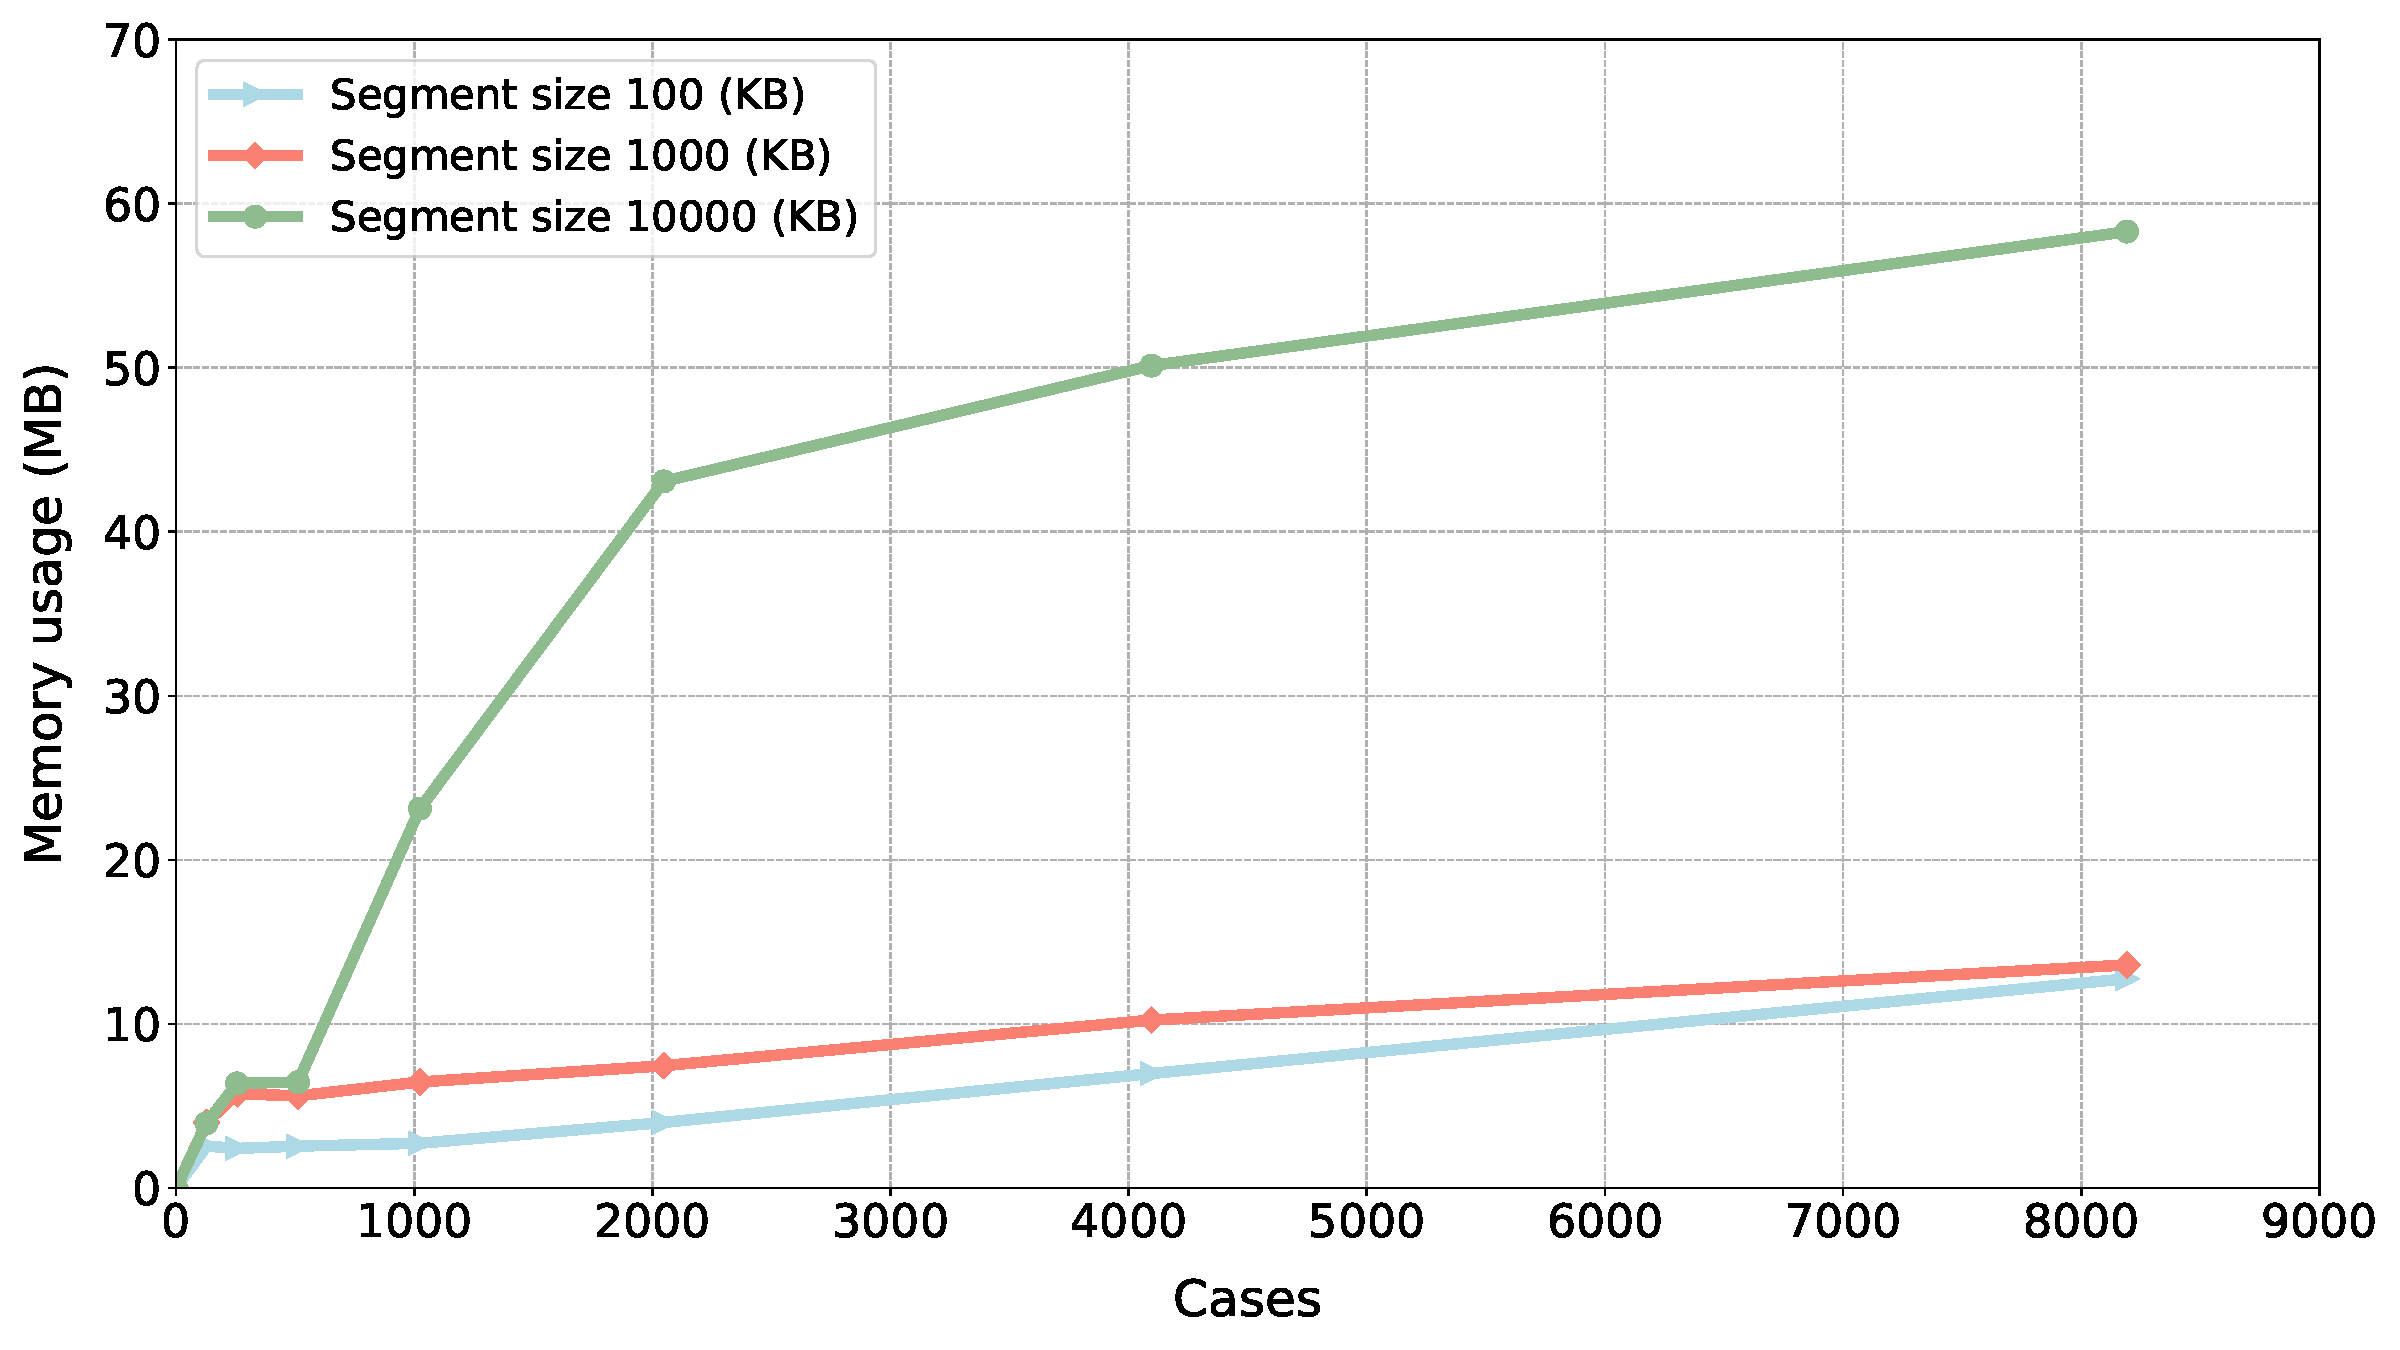
\includegraphics[width=\textwidth]{content/figures/numtraces.pdf}
  \caption{to be replaced with scalability test}
  \label{fig:cases_results}
\end{subfigure}

\begin{subfigure}{0.49\textwidth}   
  \centering
  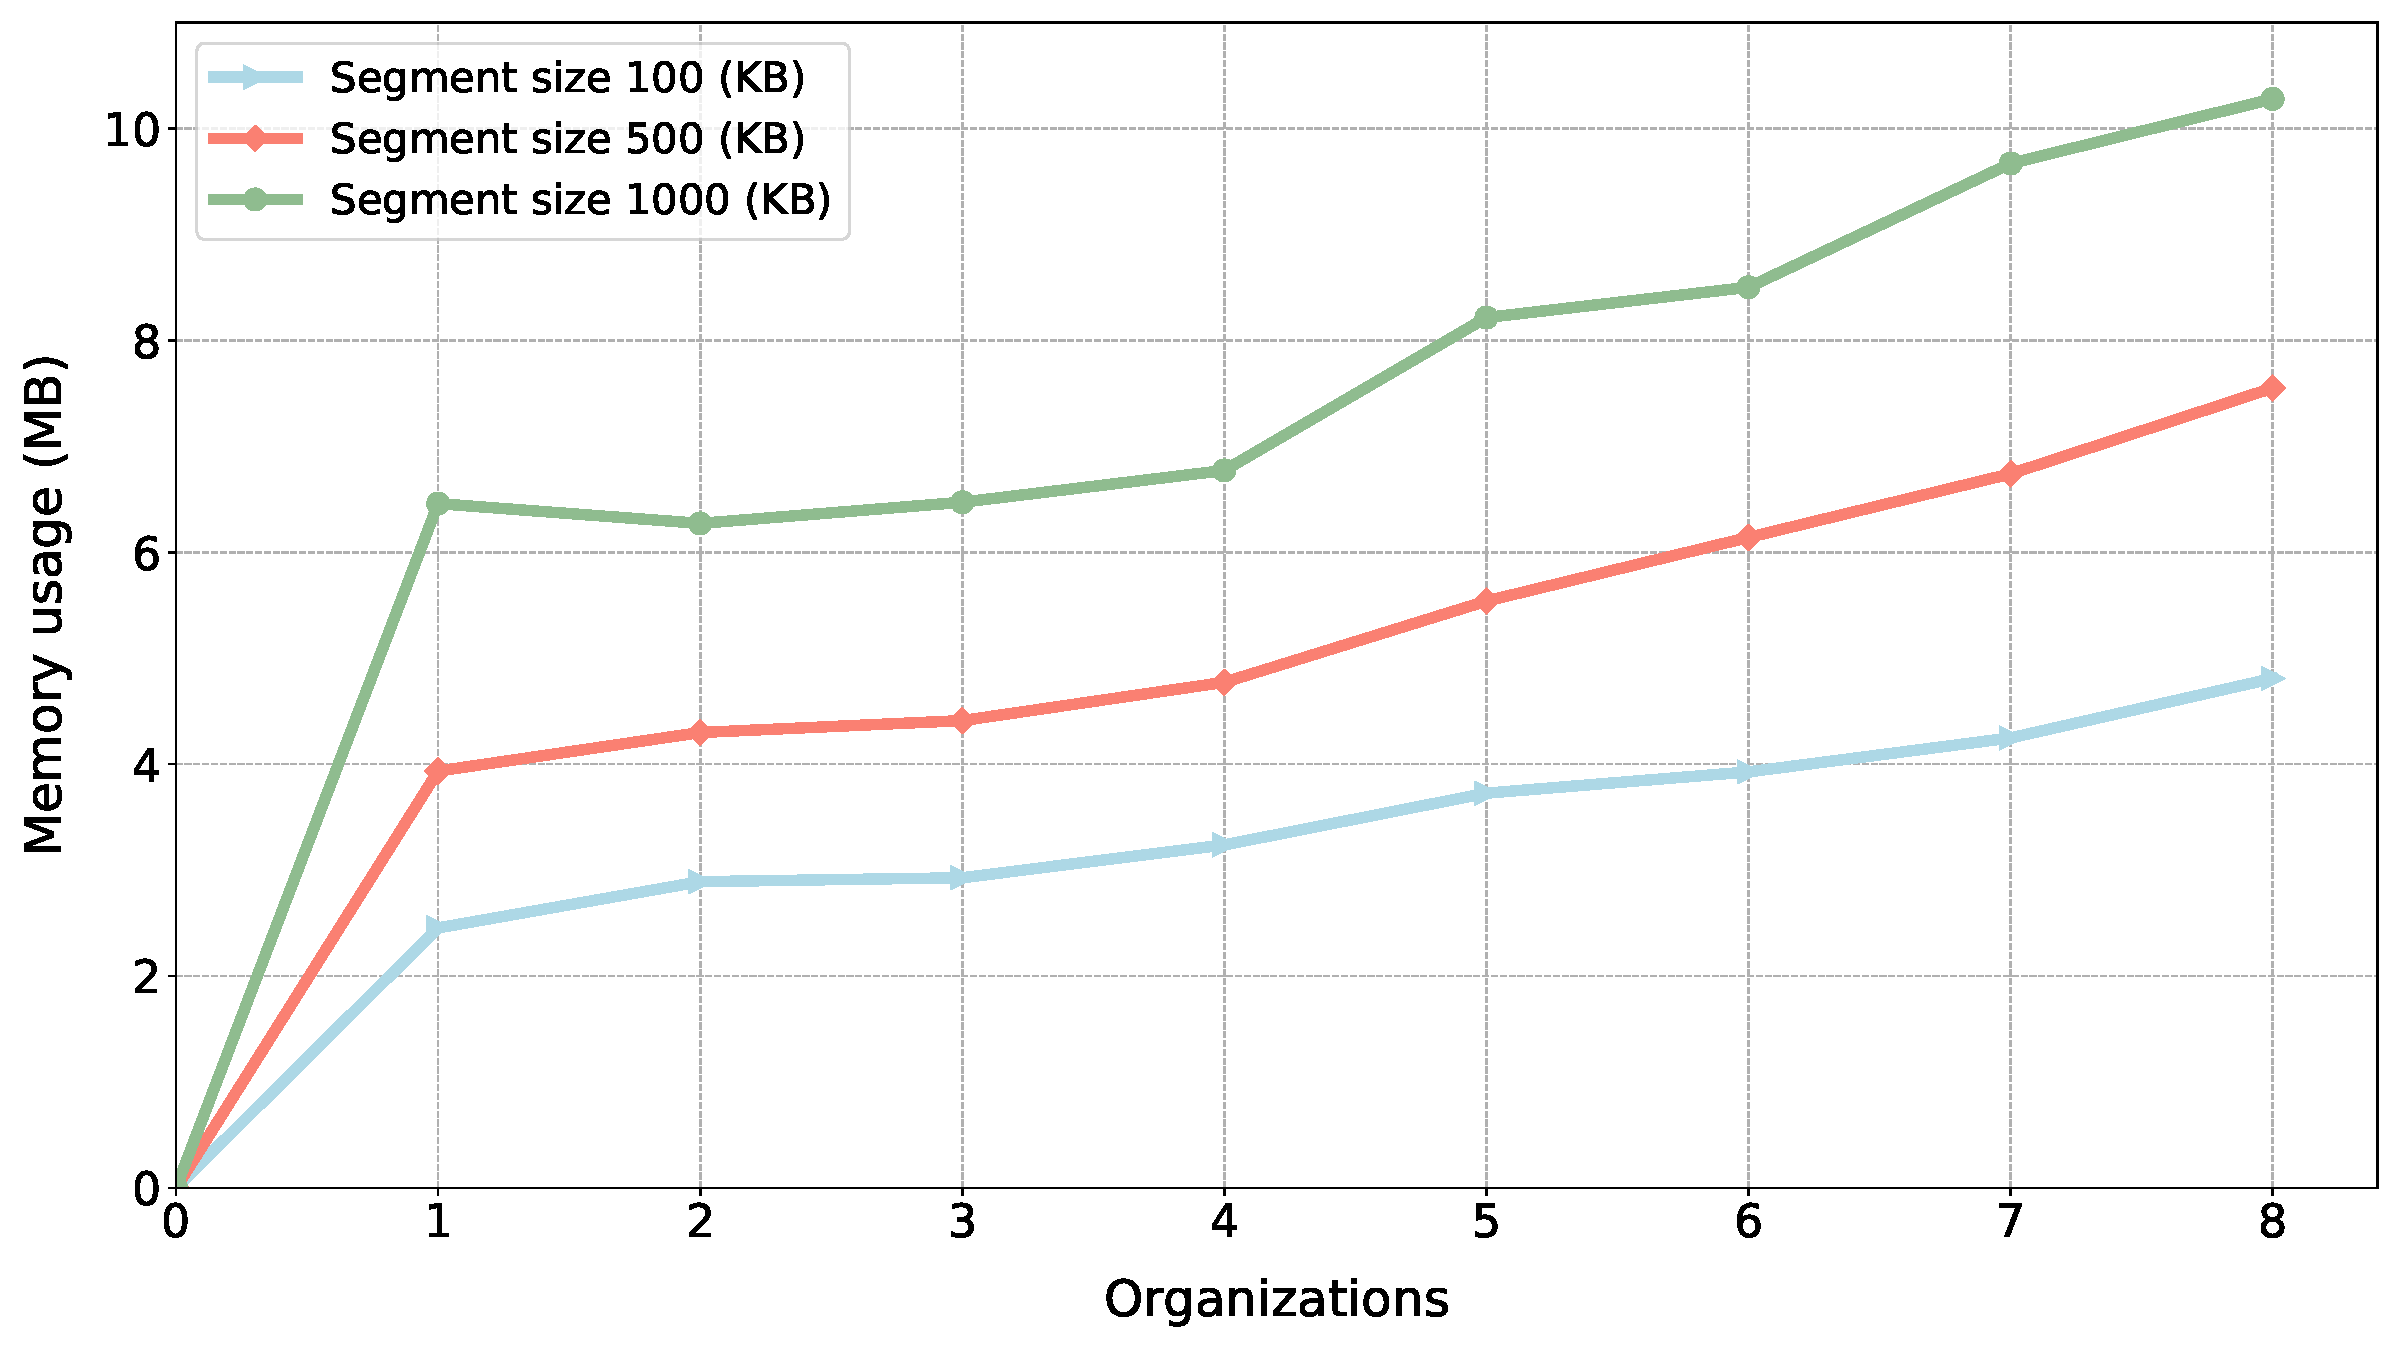
\includegraphics[width=\textwidth]{content/figures/organizationstest.pdf}
  \caption{to be replaced with scalability test}
  \label{fig:org_results}
\end{subfigure}
\begin{subfigure}{0.49\textwidth}
  \centering
   \resizebox{0.97\textwidth}{!}{%
    \begin{tabular}{l l >{\hspace{0.8em}}c>{\hspace{0.5em}} c>{\hspace{0.5em}} c}
       \toprule
         \textbf{Test} & \textbf{Seg.size} & %\textbf{Pearson}
         \textbf{$\mathbf{\rho}$} & %\textbf{Lin.Slope
         \textbf{$\mathbf{\Slope}$}& 
         %\textbf{Log. R$^2$}
         \textbf{$\mathbf{R^2}$}\\
         \midrule
         \multirow{3}{*}{\makecell[l]{Max\\events}} &
           100&0.9923& 0.0980&0.8291\\
         & 1000&0.9769&0.0821&0.9043\\
         & 10000&0.8577&0.1518&0.9386\\
         \midrule
         \multirow{3}{*}{\makecell[l]{Number\\of\\cases}} &
           100& 0.9948&0.0013&0.6822\\
         & 1000&0.9812&0.0010&0.8682\\
         & 10000&0.8791&0.0068&0.9303\\
         \midrule
         \multirow{3}{*}{\makecell[l]{Provisioning\\organizations}} &
           100 &0.9884&0.3184&0.8577\\
         & 500 &0.9799&0.5174&0.7902\\
         & 1000 &0.9521&0.6102&0.6977\\
         \bottomrule
    \end{tabular}
    }
  \label{table:TestCoefficentTable}
  \caption{Scalability metrics results}
\end{subfigure}
\caption{Memory usage and scalability test results}
\label{os}
\end{figure}

\end{comment}

\begin{figure}[t]
	\begin{subfigure}{0.49\textwidth}   
		\centering
		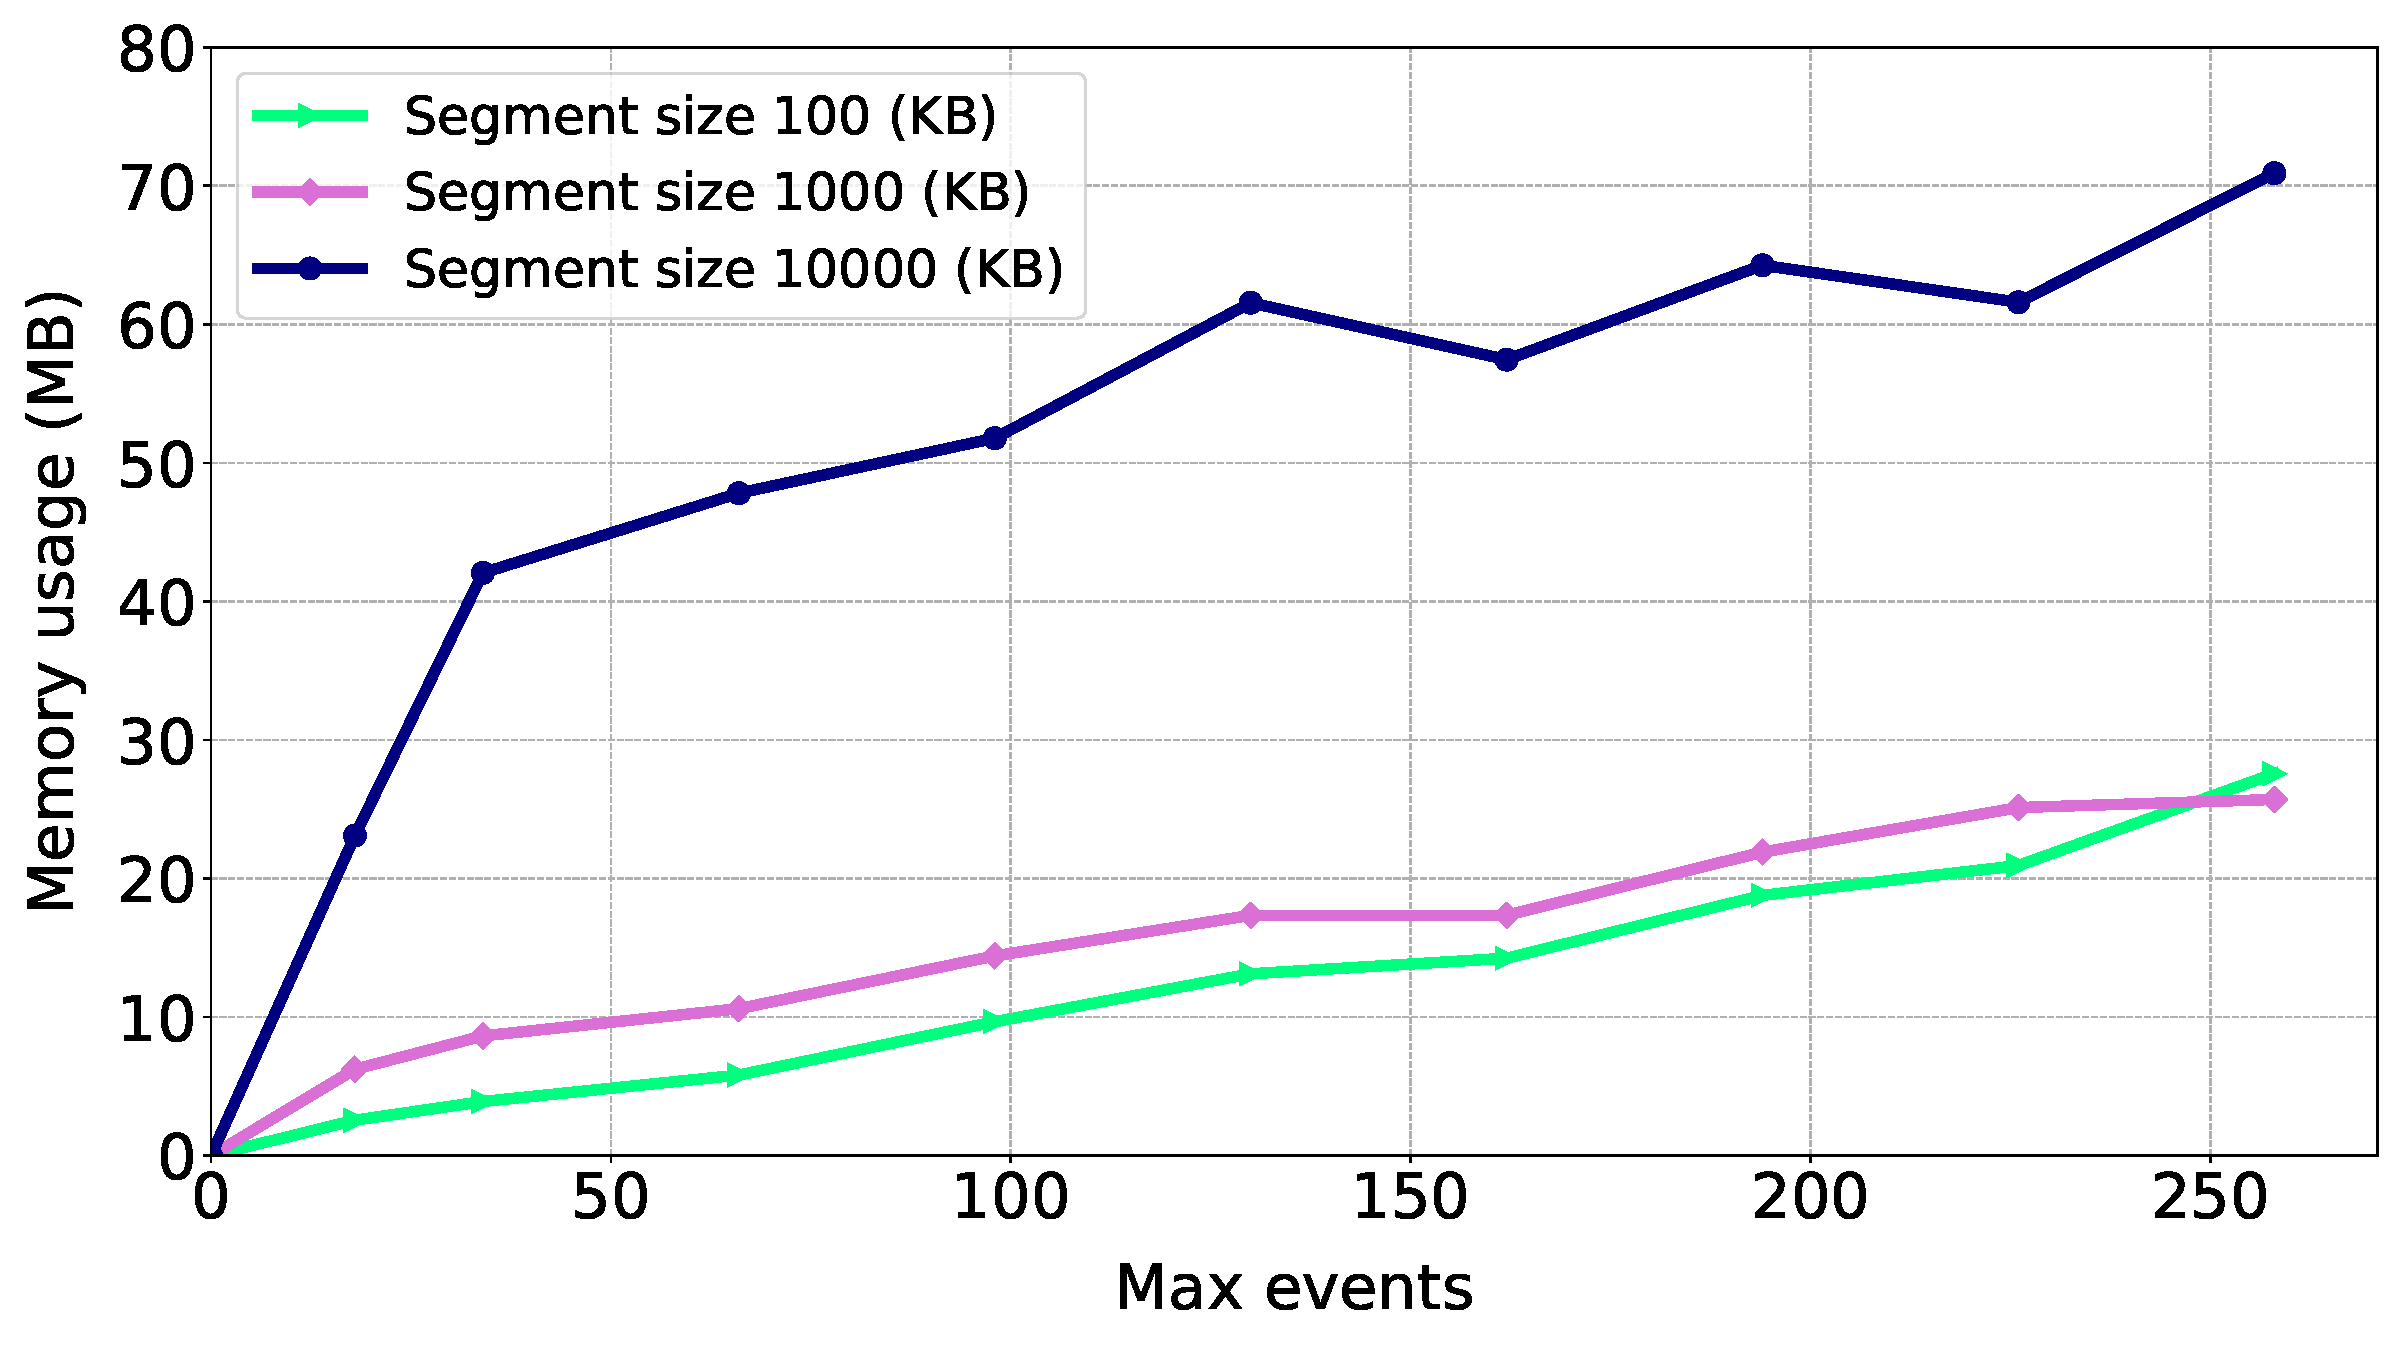
\includegraphics[width=\textwidth]{content/figures/maxevents-2.pdf}
		\caption{Results of scalability test \ref{test:events}}
		\label{fig:event_results}
	\end{subfigure}
	\begin{subfigure}{0.49\textwidth}   
		\centering
		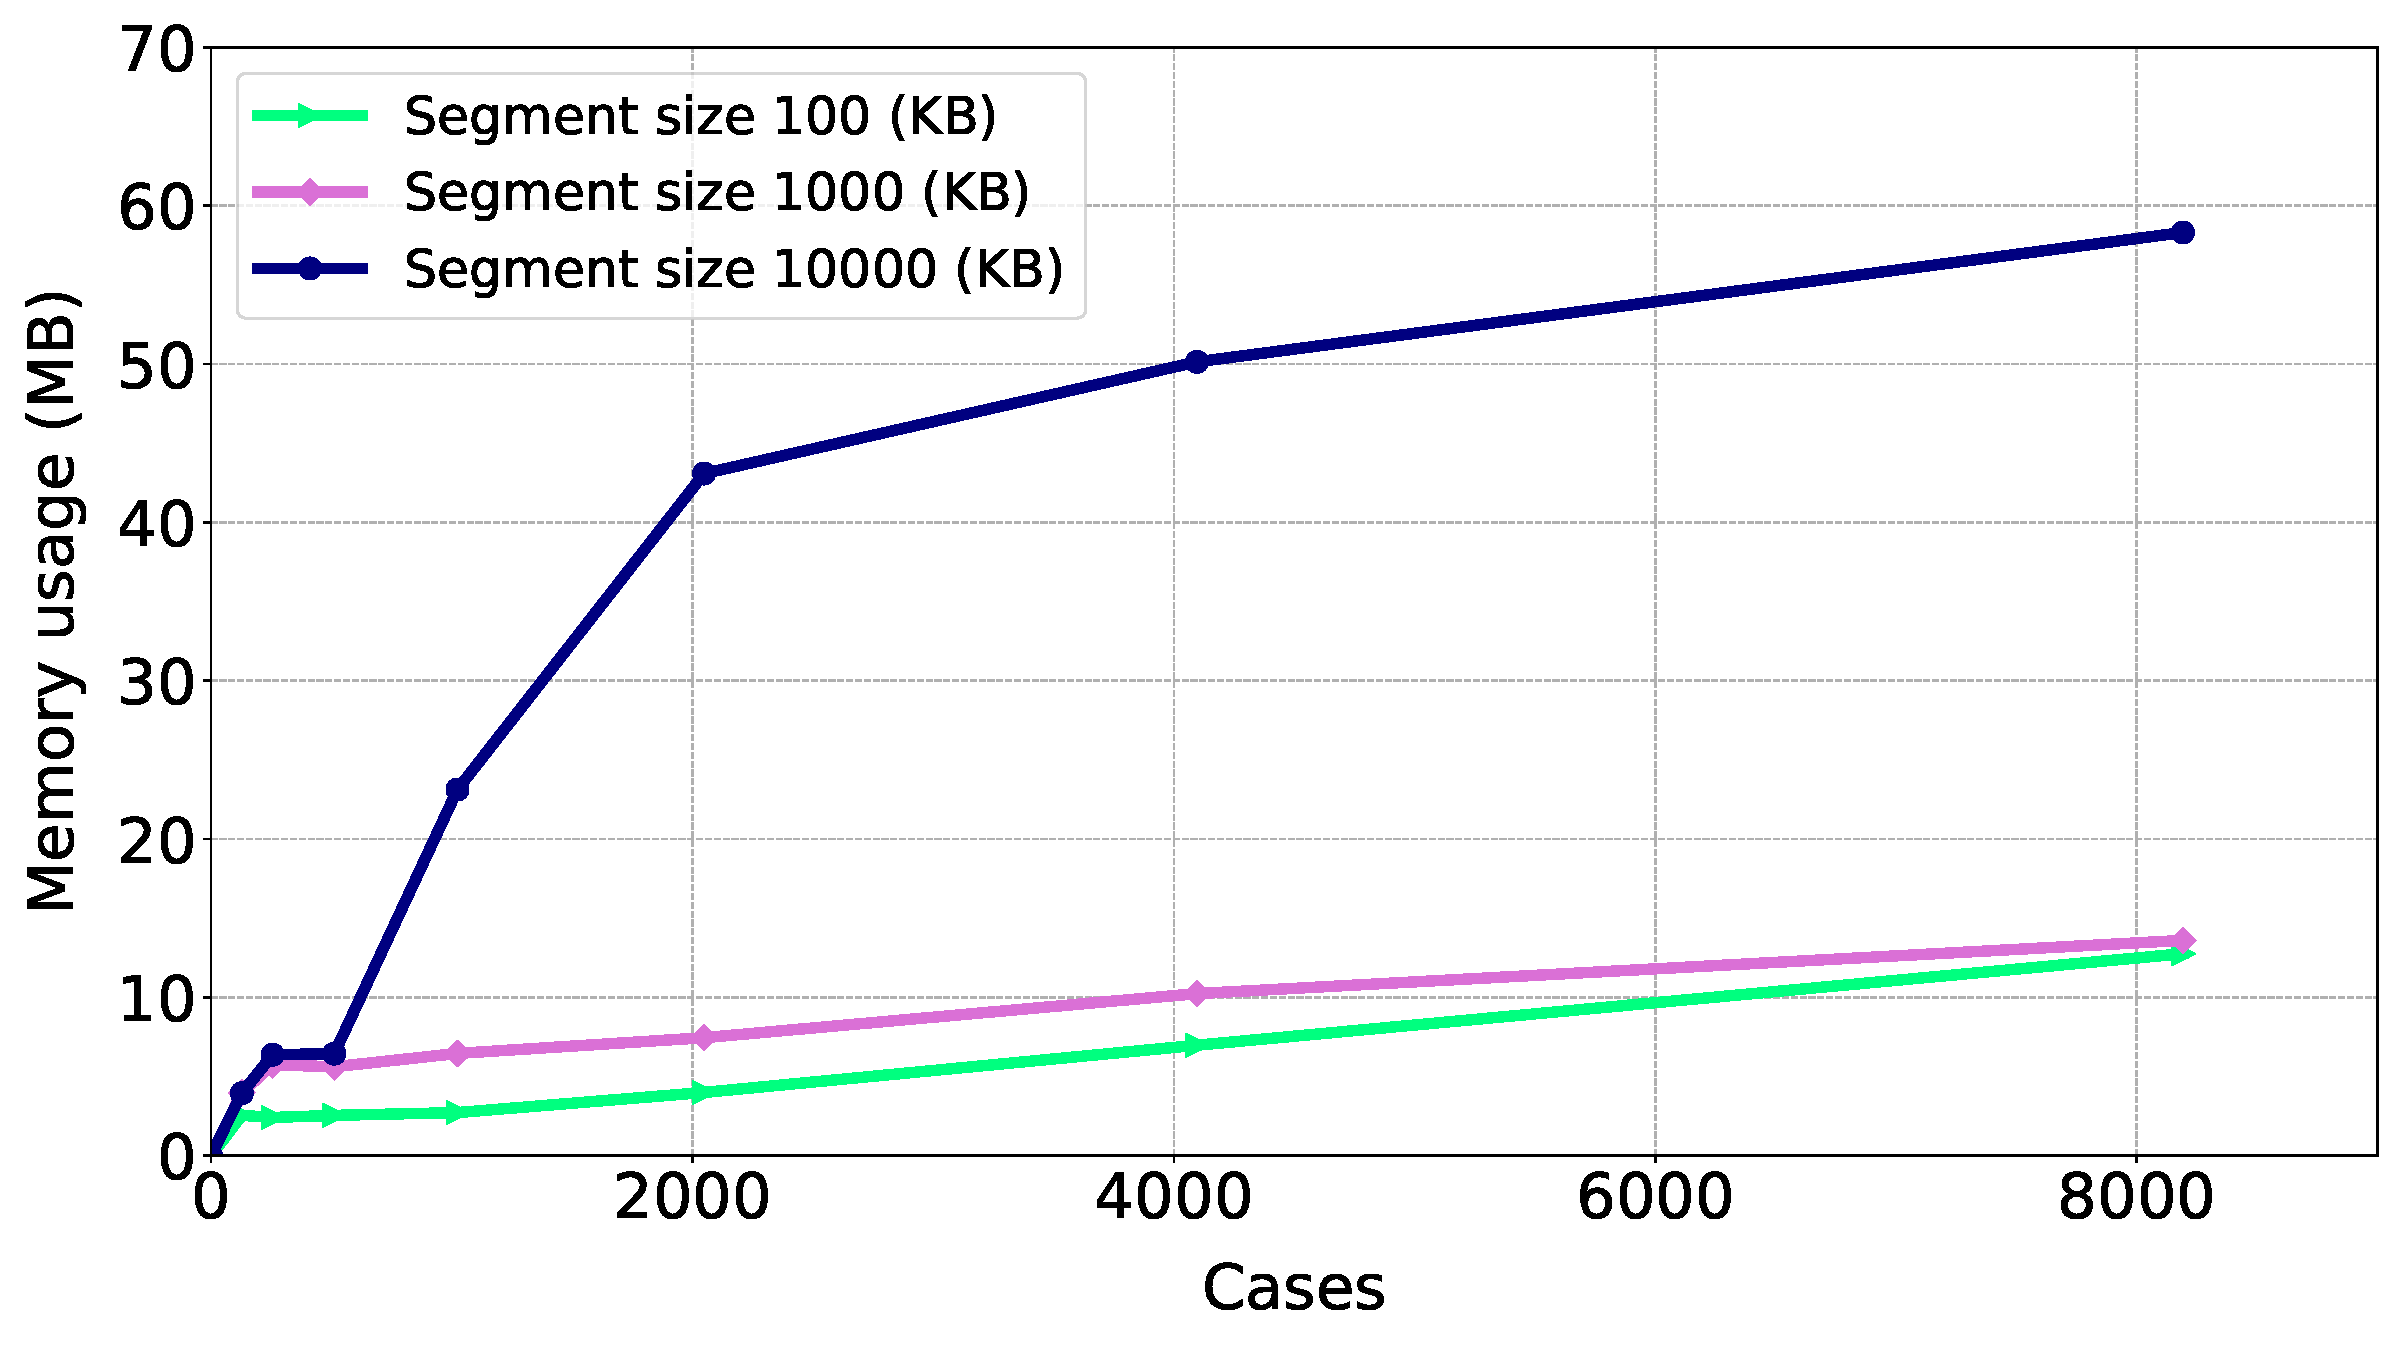
\includegraphics[width=\textwidth]{content/figures/numtraces-2.pdf}
		\caption{Results of scalability test \ref{test:cases}}
		\label{fig:cases_results}
	\end{subfigure}
	
	\begin{subfigure}{0.49\textwidth}   
		\centering
		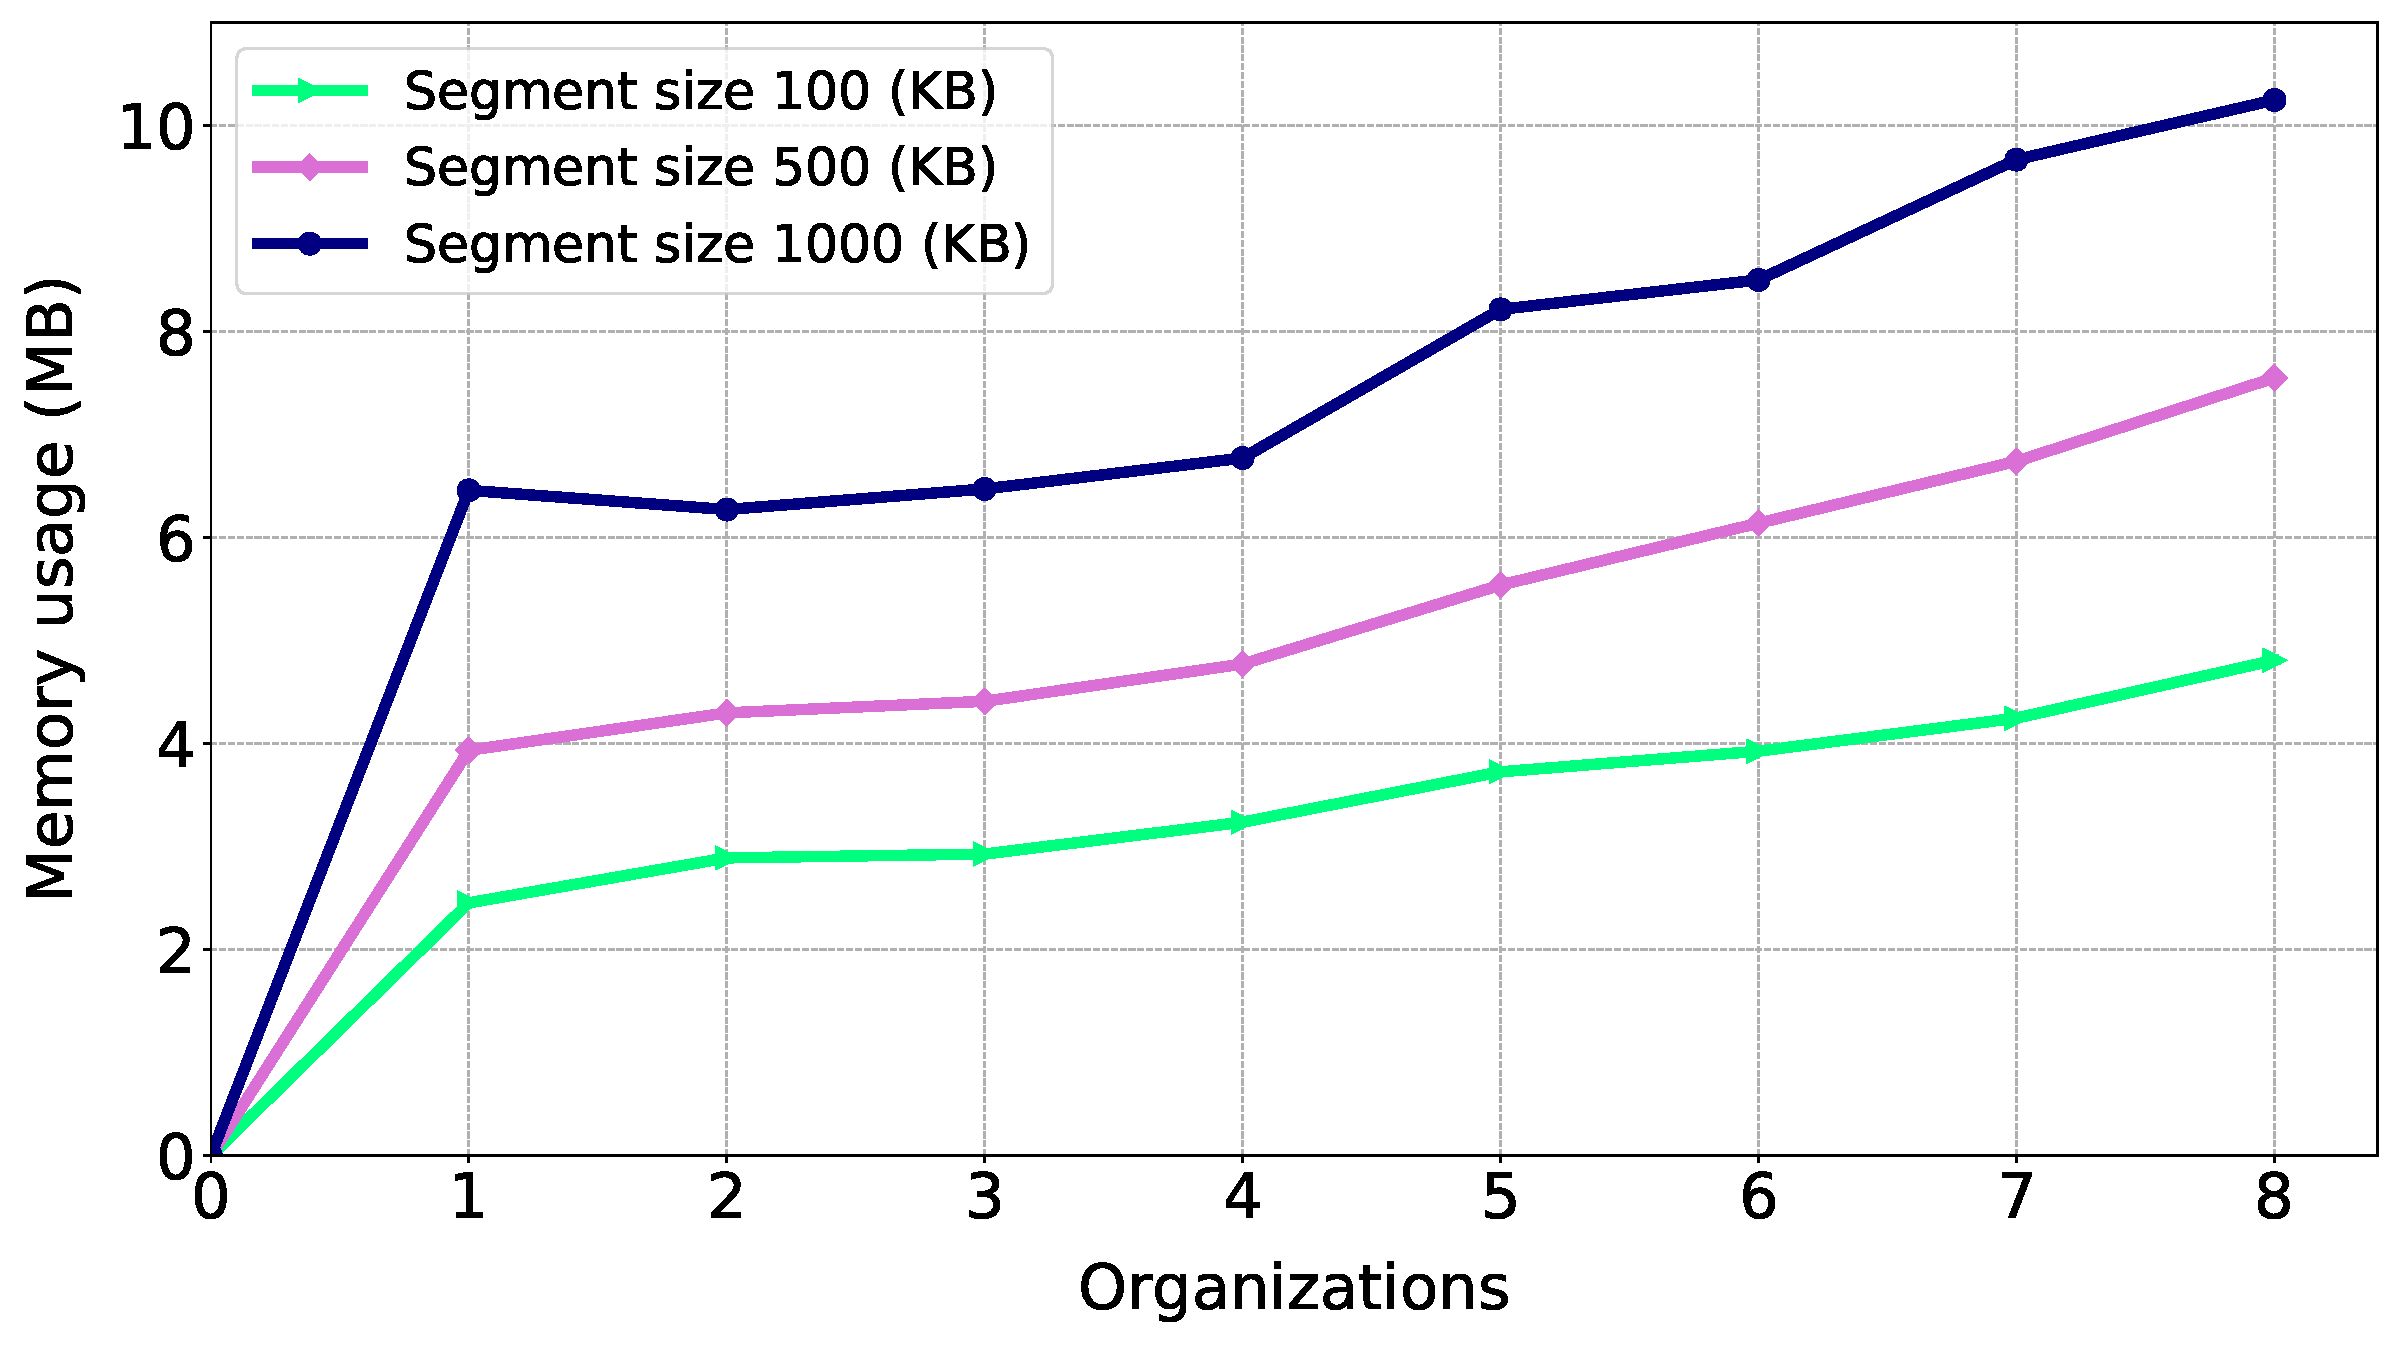
\includegraphics[width=\textwidth]{content/figures/organizationstest-2.pdf}
		\caption{Results of scalability test \ref{test:organizations}}
		\label{fig:org_results}
	\end{subfigure}
	\begin{subtable}{0.49\textwidth}
		\centering
		\resizebox{0.97\textwidth}{!}{%
			   %l l >{\hspace{1em}}c>{\hspace{0.2em}} c>{\hspace{0.8em}} c
	\begin{tabular}{ll>{\hspace{1em}}cc>{\hspace{1em}}c}
	\toprule
	\textbf{Test} & \textbf{Seg.size} & %\textbf{Pearson}
	\textbf{\Rlin} & %\textbf{Lin.Slope
		\textbf{$\Slope$}& 
		$\Rlog$\\
		\midrule
		\multirow{3}{*}{\makecell[l]{Max\\events}} &
		100&0.9847& 0.0980&0.8291\\
		& 1000&0.9544&0.0821&0.9043\\
		& 10000&0.7357&0.1518&0.9386\\
		\midrule
		\multirow{3}{*}{\makecell[l]{Number\\of\\cases}} &
		100&0.9896&0.0013&0.6822\\
		& 1000&0.9629&0.0010&0.8682\\
		& 10000&0.7729&0.0068&0.9303\\
		\midrule
		\multirow{3}{*}{\makecell[l]{Provisioning\\organizations}} &
		100 &0.9770&0.3184&0.8577\\
		& 500 &0.9602&0.5174&0.7902\\
		& 1000 &0.9066&0.6102&0.6977\\
		\bottomrule
	\end{tabular}

		}
		\label{table:TestCoefficentTable}
		\caption{Scalability measurements}
	\end{subtable}
	\caption{Scalability test results}
	\label{fig:scalabtest}
\end{figure}
\noindent\textbf{Scalability.}
In this subsection, we examine the scalability of the \Compo{Secure Miner}, focusing on its capacity to efficiently manage an increasing workload in the presence of limited memory resources. We implemented three distinct test configurations gauging runtime memory usage as variations of our motivating scenario log. In particular, we considered
\begin{inparaenum}[(I)]
	\item\label{test:events} the maximum number of events per case,
	\item\label{test:cases} the number of cases $|{\CIdU}|$, and 
	\item\label{test:organizations} the number of provisioning organizations $|{\OrgU}|$
\end{inparaenum}
as independent integer variables. To conduct the test on the maximum number of events, we added a loop back from the final to the initial activity of the process model, progressively increasing the number of iterations $2 \leqslant \,x_\circlearrowleft\, \leqslant 16$ at a step of \num{2}, resulting in $18+16\cdot(x_\circlearrowleft-1)$ events. Concerning the test on the number of cases, we simulated additional process instances so that $|{\CIdU}| = 2^{x_{\CId}}$ having $x_{\CId} \in \{7,8,\ldots,13\}$. Finally, for the assessment of the number of organizations, the test necessitated the distribution of the process model activities' into a variable number of pools, each representing a different organization ($|{\OrgU}| \in \{1,2,\ldots,8\}$).
%
We parameterized the above configurations with three segment sizes (in KiloBytes): $\SegSize \in \{100,1000,10000\}$ for tests \ref{test:events}~and~\ref{test:cases}, and $\SegSize \in \{100,500,1000\}$ for test~\ref{test:organizations} (the range is reduced without loss of generality to compensate the partitioning of activities into multiple organizations). To facilitate a more rigorous interpretation of the output trends across varying {\SegSize} configurations, we employ 
two well-known statistical measures. As a primary measure of goodness-of-fit, we employ the coefficient of determination {\RCoefficent}~\citep{barrett1974coefficient}, which assesses the degree to which the observed data adheres to the linear ({\Rlin}) and logarithmic ({\Rlog}) regressions derived from curve fitting approximations. To further delve into the analysis of trends with a high {\Rlin}, we consider the slope {\Slope} of the approximated linear regression~\citep{altman2015simplelinearregression}. 
\begin{comment}
Given two sequences of values $\langle x_1,\ldots, x_k \rangle$ and $\langle y_1, \ldots, y_k \rangle$ with $k \in \mathbb{N}$, the measures are computed as follows:
\begin{center}
	\begin{minipage}{.5\linewidth}
		\begin{equation}
			\RCoefficent = \RCoefficentF;
		\end{equation}
	\end{minipage}%
	\begin{minipage}{.5\linewidth}
		\begin{equation}
			\Slope = \SlopeF.
		\end{equation}
	\end{minipage}
\end{center}
\end{comment}

%a comprehensive set of metrics outlined in \cref{formula}. 
% Subsequently, we utilized the measurements listed in 
%Table~\ref{fig:scalabtest}(d) 
\hyperref[table:TestCoefficentTable]{Table 9(d)} lists the measurements we obtained. We describe them to elucidate the observed patterns. \Cref{fig:event_results} depicts the results of test \ref{test:events}, focusing on the increase of memory utilization when the number of events in the event logs grows. We observe that the memory usage for {\SegSize} \num{100} and \num{1000} (depicted by green and lilac lines, respectively) are quite similar, whereas the setting with {\SegSize} \num{10000} (blue line) exhibits significantly higher memory usage. For the settings with {\SegSize} \num{100} and \num{1000}, {\Rlin} approaches \num{1}, %(\num{0.9847} and \num{0.9544} respectively), 
signifying an almost perfect approximation of the linear relation, against lower {\Rlog} values. % (\num{0.8291} and \num{0.9043}, respectively). 
In these test settings, {\Slope} is very low %(\num{0.0980} and \num{0.0821}, respectively) 
yet higher than \num{0}, thus indicating that memory usage is likely to continue increasing as the number of max events grows. The configuration with {\SegSize} \num{10000} yields a higher {\Rlog} value, % (\num{0.9386}), 
thus suggesting a logarithmic trend, hence %a better logarithmic approximation and suggesting 
a greater likelihood of stabilizing memory usage growth rate as the number of maximum events increases. 
%
In  \cref{fig:cases_results}, we present the results of test \ref{test:cases}, assessing the impact of the number of cases on the memory consumption. As expected, the configurations with {\SegSize} set to \num{100} and \num{1000} exhibit a trend of lower memory usage than settings with {\SegSize} \num{10000}. The {\Rlin} score of the trends with {\SegSize} \num{100} and \num{1000} %(0.9896 and 0.9629, respectively) 
indicate a strong linear relationship between the dependent and independent variables compared to the trend with {\SegSize} \num{10000}, which is better described by a logarithmic regression (${\Rlog} = \num{0.9303}$). For the latter, the {\Rlog} value is higher than the corresponding {\Rlin} %(0.7729) 
thus suggesting that the logarithmic approximation is better suited to describe the trend. %, thus implying a higher likelihood of growth rate stabilization as the number of cases increases. 
Differently from test \ref{test:events}, the {\Slope} score associated with the linear approximations of the trends with {\SegSize} \num{100} and \num{1000} %(\num{0.0013} and \num{0.0010}, respectively) 
approaches \num{0}, indicating that the growth rate of memory usage as the number of cases increases is negligible.
%
In \cref{fig:org_results}, we present the results of test~\ref{test:organizations}, on the relation between the number of organizations and the memory usage. The chart shows that memory usage trends increase as provisioning organizations increase for all three segment sizes. The {\Rlin} values for the three {\SegSize}s are very high, %(\num{0.9770}, \num{0.9602}, and \num{0.9066}, from the lower to the higher \SegSize), 
indicating a strong positive linear correlation. % between the number of organizations and memory usage. 
The test with {\SegSize} \num{100} exhibits the slowest growth rate, as corroborated by the lowest {\Slope} result (\num{0.3184}). 
For the configuration with {\SegSize} \num{500}, the memory usage increases slightly faster (${\Slope} = {0.5174}$). With {\SegSize} \num{1000}, the overall memory usage increases significantly faster than the previous configurations (${\Slope} = 0.6102$). We derive from these findings that the \Compo{Secure Miner} may encounter scalability issues when handling settings with a large number of provisioning organizations. Further investigation is warranted to determine the precise cause of this behavior and identify potential mitigation strategies. 

In the next section, we conclude our work and outline future research directions based upon our current findings and the limitations of our approach.
